\documentclass[10pt,a4paper,twoside]{book}

% UNICORNS %
\usepackage[british]{babel}
\usepackage{combelow}
\useshorthands{"}
\defineshorthand{"s}{\cb{s}}

% packages
\usepackage{adjustbox}
\usepackage{geometry}
\usepackage{fancyhdr}
\usepackage{url}
\usepackage{amsmath}
\usepackage{amssymb}
\usepackage[algochapter]{algorithm2e}
\usepackage{listings}
\usepackage[usenames, dvipsnames]{color}
\usepackage{algorithmic} 
%\usepackage{lipsum}
% end packages

\usepackage{color}
\definecolor{lightgray}{rgb}{.9,.9,.9}
\definecolor{darkgray}{rgb}{.4,.4,.4}
\definecolor{purple}{rgb}{0.65, 0.12, 0.82}

\lstdefinelanguage{JavaScript}{
  keywords={typeof, new, true, false, catch, function, return, null, catch, switch, var, if, in, while, do, else, case, break},
  keywordstyle=\color{blue}\bfseries,
  ndkeywords={class, export, boolean, throw, implements, import, this},
  ndkeywordstyle=\color{darkgray}\bfseries,
  identifierstyle=\color{black},
  sensitive=false,
  comment=[l]{//},
  morecomment=[s]{/*}{*/},
  commentstyle=\color{purple}\ttfamily,
  stringstyle=\color{red}\ttfamily,
  morestring=[b]',
  morestring=[b]"
}

\lstset{
   language=JavaScript,
   backgroundcolor=\color{lightgray},
   extendedchars=true,
   basicstyle=\small\ttfamily,
   showstringspaces=false,
   showspaces=false,
   numbers=left,
   numberstyle=\footnotesize,
   numbersep=10pt,
   tabsize=4,
   breaklines=true,
   showtabs=false,
   captionpos=b,
   xleftmargin=0.7cm,
   aboveskip=1.5em
}


% configure style of pages

\geometry{a4paper,lmargin=2.54cm,rmargin=2.54cm,tmargin=2.54cm,bmargin=2.54cm}

\renewcommand{\baselinestretch}{1}

\fancypagestyle{plain}{
  \fancyhf{}

  \renewcommand{\headrulewidth}{0.5pt}
  \renewcommand{\footrulewidth}{0.5pt}

  \fancyfoot[C]{\thepage}
}

\fancypagestyle{marked}{
  \fancyhf{}

  \renewcommand{\headrulewidth}{0.5pt}
  \renewcommand{\footrulewidth}{0.5pt}

  \fancyhead[LO]{\slshape \rightmark}
  \fancyhead[RE]{\slshape  \leftmark}

  \fancyfoot[C]{\thepage}
}

\pagestyle{plain}


\begin{document}

% =============================================================================
% Title page

 \newpage
  \thispagestyle{empty}

    \adjustbox{padding={5pt},frame={1pt},right}{Dissertation Type: research}

  \vspace*{\fill}
  \begin{center}
                
\includegraphics[scale=0.3]{logo/logo_uob_color}                \\
                              \vspace*{1.0cm}
                          DEPARTMENT OF COMPUTER SCIENCE                        \\
                              \vspace*{2.0cm}
                       
 				 \mbox{{\LARGE Side-Channel Attacks in Web Browsers}} \\
                              \vspace*{0.5cm}
                              \vspace*{1.0cm}
                          {\Large Ana-Maria Dumitra"s}                         \\

                              \vspace*{1.0cm}
                          \rule{0.5\textwidth}{0.5pt}
                              \vspace*{1.0cm}

            A dissertation submitted to the University of Bristol
            in accordance with the requirements of the degree of
            Master   of Engineering
                    in the Faculty of Engineering.                                

                              \vspace*{1.0cm}
                          \rule{0.5\textwidth}{0.5pt}
                              \vspace*{1.0cm}

                                  \today
  \end{center}
  \vspace*{\fill}
  
%==============================================================================
% Front matter

\cleardoublepage
\pagestyle{plain}
\pagenumbering{roman}

% =============================================================================
% Declaration

\newpage
  \thispagestyle{plain}

  \chapter*{Declaration}

  This dissertation is submitted to the University of Bristol in accordance 
  with the requirements of the degree of MEng in the Faculty 
  of Engineering.  It has not been submitted for any other degree or diploma 
  of any examining body.  Except where specifically acknowledged, it is all 
  the work of the Author. 

  \vspace{6cm}

  \noindent {Ana-Maria Dumitra"s}, \today


\tableofcontents
\listoffigures
\listoftables
\listofalgorithms
\lstlistoflistings

%========================================================================================================

% -----------------------------------------------------------------------------


\chapter*{Executive Summary}

This dissertation is about side-channel attacks in the browser, a very powerful category of side-channel attacks which affect browser software and whose aim is to disclose private data about the user through either using timing information (\textit{Timing Attacks}) or the state of the browser's cache memory (\textit{Cache Attacks}). 
\\\\
\noindent
The world of browser attacks is rapidly changing, with new vulnerabilities appearing and disappearing within weeks. In general, adversaries have a limited time frame in which they can exploit the vulnerability; however, some side-channel attacks in the browser have been around for decades. This is due to the fact that fixing the vulnerability will bring severe performance penalties to the browser software. The relatively short life span of these types of attacks, motivated me to investigate if some of the attacks released over the past year are still possible.  
\\\\
\noindent
Throughout this paper we look at two types of browser side-channel attacks: \textit{cache attacks}, which analyse the state of the browser's cache memory in order to disclose private information about users, such as their browsing activity, and \textit{timing attacks}, which use timing information to reveal a user's browsing history or gain access to their view of a cross-origin website.

\section*{Main Achievements}

\begin{itemize}
\item I analysed the effectiveness of some of the most popular browser side-channel attacks over the past twenty years. The results are presented in Chapter \ref{chap:realtedWork}.
\item I implemented a recently released cache attack in the browser and tested if it is still possible.
\item I evaluated the measuring techniques proposed by Van Goethem et al. \cite{van2015clock} and tested their performance against previous methods. 
\item I built several web applications which assess the efficiency of the measuring methods presented by Van Goethem et al. \cite{van2015clock}.
\end{itemize}

% -----------------------------------------------------------------------------

\chapter*{Supporting Technologies}

\begin{quote}
\noindent
\begin{itemize}
\item I use HTML \cite{berjon2014html} , CSS \cite{cssdoc}, JavaScript \cite{jsdoc} and AngularJS\cite{angularjs} for building the web applications.
\item I use Google Chart Angular \cite{googlechartsangular} and Google Charts \cite{googlecharts} in order to plot the graphs.
\end{itemize}
\end{quote}

% -----------------------------------------------------------------------------

\chapter*{Notation and Acronyms}

% {\bf An optional section, of roughly $1$ or $2$ pages}
% \vspace{1cm} 

% \noindent
% Any well written document will introduce notation and acronyms before
% their use, {\em even if} they are standard in some way: this ensures 
% any reader can understand the resulting self-contained content.  

% Said introduction can exist within the dissertation itself, wherever 
% that is appropriate.  For an acronym, this is typically achieved at 
% the first point of use via ``Advanced Encryption Standard (AES)'' or 
% similar, noting the capitalisation of relevant letters.  However, it 
% can be useful to include an additional, dedicated list at the start 
% of the dissertation; the advantage of doing so is that you cannot 
% mistakenly use an acronym before defining it.  A limited example is 
% as follows:

\begin{quote}
\noindent
\begin{tabular}{lcl}
% AES                 &:     & Advanced Encryption Standard                                         \\
% DES                 &:     & Data Encryption Standard                                             \\
%                     &\vdots&                                                                      \\
% ${\mathcal H}( x )$ &:     & the Hamming weight of $x$                                            \\
% ${\mathbb  F}_q$    &:     & a finite field with $q$ elements                                     \\
% $x_i$               &:     & the $i$-th bit of some binary sequence $x$, st. $x_i \in \{ 0, 1 \}$ \\

AES			   	 	&:	   & Advanced Encryption Standard							 \\	
API					&:     & Application Program Interface							 \\
AppCache		   	 	&:	   & Application Cache   									 \\	
CPU					&:	   & Central Processing Unit									 \\
CRT					&:	   & Chinese Remainder Theorem								 \\
CSS					&:	   & Cascading Style Sheets									 \\
DES					&:	   & Data Encryption Standard								 \\
DRAM					&:	   & Dynamic Random Access Memory							 \\
HTML					&:     & HyperText Markup Language								 \\
LLC					&:	   & Last-Level Cache										 \\
RAM					&:	   & Random Access Memory									 \\
RSA					&:	   & Rivest-Shamir-Adleman Cryptosystem				    		 \\
SCA					&:	   & Side-Channel Attack										 \\	
SRAM					&:	   & Static Random Access Memory								 \\
\end{tabular}
\end{quote}

% -----------------------------------------------------------------------------

\chapter*{Acknowledgements}

\noindent
Firstly, I would like to thank my supervisor, Dr. Elisabeth Oswald, for her valuable feedback, help and guidance throughout this project. This project would not had been possible without her support and advice. 

I would like to thank my family for their love and support. Additionally, thanks are owed to my friends for making numerous trips to the Clifton Suspension Bridge.

Finally, I would like to thank the people in MVB 2.09 ("The Back Lab") for providing great advice and making the past 96 days somewhat more bearable. Special thanks must go to Richard Grafton for getting us a sofa.




%========================================================================================================
% Main matter
\cleardoublepage
\pagestyle{marked}
\pagenumbering{arabic}
\parindent=0in
\parskip=1em 

%%%%%%%%%%%%%%%%%%%%%%%%%%%%%%%%%%%%%%%%%%%%%%%%%%%%%%%%%%%%%%%%%%%%%%%%%%%%%%%%%%%%%%%%%%%%%%%%%%%%%%%%%
%%%%%%%%%%%%%%%%%%%%%%%%%%%%%%%%%%%%%%%%%%%%%% UNICORNS %%%%%%%%%%%%%%%%%%%%%%%%%%%%%%%%%%%%%%%%%%%%%%%%%
%%%%%%%%%%%%%%%%%%%%%%%%%%%%%%%%%%%%%%%%%%%%%%%%%%%%%%%%%%%%%%%%%%%%%%%%%%%%%%%%%%%%%%%%%%%%%%%%%%%%%%%%%

% -----------------------------------------------------------------------------

\chapter{Contextual Background}
\label{chap:context}

\section{Topic Background}

The focus of this project are Side-Channel attacks in the browser. Browser attacks are a category of side-channel attacks which target vulnerabilities in the browser software. The aim of this particular kind of attacks is to disclose private data about users by analysing unintentional information leakage.

\subsection{Side-Channel Attacks}
Timing information, power consumption, electromagnetic emission or heat dissipation measured while the device performs an interesting operation can reveal sensitive information. These leaks, based on physical characteristics are known as \textit{Side Channels}. Side-Channel Attacks (SCA) are a powerful set of attacks which rely on recovering secret data by analysing the device rather than exploiting vulnerabilities in the underlying algorithm.

Side-Channel Attacks can be split in two categories based on the goal of the attacker:
\begin{itemize}
\item Side-Channel Attacks which target faults in the implementation of cryptographic algorithm in order to recover the secret parameters used in the computation. 
\item And Side-Channel Attacks whose aim it to disclose the private information about the user, such as browsing activity or history.
\end{itemize}
In this dissertation I am going to focus on the second category and present several side-channel attacks which lead to the disclosure of a user's private data.

\subsection{Browser Attacks}
Since the invention of the Internet, over twenty years ago, there has been an increase in the number of web based applications. The creation of the Infrastructure as a Service (IaaS) platforms, such as Amazon Elastic Compute Cloud (EC2)\cite{ec2} and the Google App Engine (GAE)\cite{gae}, made the process of running and maintaining web based applications a lot easier. This, not only determined companies to move their business online, but also influenced the development of new web technologies and motivated browser vendors to add more and more features to their software. 

Newer web technologies and updated browsers not only improved the overall user experience and eased the development process, but also opened the way for a new series of attacks, known as browser attacks. One interesting fact about browser attacks is that new vulnerabilities emerge every day, but they also disappear within weeks, which gives adversaries a limited time frame in which they can exploit potential vulnerabilities in web software. It is very rare that vulnerabilities in browser software and web development technologies last more than a year.

Browser attacks fell into two categories: traditional timing attacks, which measure the server's response time in order to derive meaningful information about the state of the website, and cache timing attacks, which investigate the state of the browser's cache memory through measuring the access time of various resources in order to determine if they have been cached or not.

\section{Motivation}

Browser attacks are an important category of side channel attacks which affect a large number of people. In general, these type of attacks require minimal set up. A user simply has to navigate to an untrusted web page, which contains attacker-controlled content. The website runs a script in the background, that collect side channel information which will later be used to disclose private data about the user. Most of the time the user is unaware of what is happening in the background.

The goal of an attacker in browser side-channel attacks is to disclose private data about the user. This information can be anything from the user's location to what pages they visited and even what pages they are currently browsing.

One might think that browser attack can be avoided by staying away from untrusted websites; however, researchers \cite{jang2010empirical} proven that even high-profile websites use browser side-channel attacks in order to obtain private data about their visitors. Various companies will use the knowledge in different ways. For example, an online store platform might want to display some targeted advertisements in order to increase the visit to purchase ratio on their website, or health insurance providers might want to gain access to what health related web pages their users have previously visited. No matter what the reason behind these attack is, they pose a serious threat to user's privacy.

\section{Aims and Objectives}
The overall goal of this project is to evaluate different browser attacks. Browser attacks are an interesting category of side-channel attack, where new vulnerabilities appear and disappear within weeks. This means that attackers have a limited time frame in which they can exploit potential side channels in the browser software. This motivated me to evaluate the efficiency of several browser attacks released during the past year. The concrete objectives of this project are:
\begin{enumerate}
\item To review some of the most popular browser attacks and see if they are still possible.
\item Implement the JavaScript Cache Timing Attack discovered by Oren et al. \cite{oren2015spy}.
\item To implement the novel measuring techniques proposed by Van Goethem et al. \cite{van2015clock}.
\item To compare the measuring techniques described by Van Goethem et al. \cite{van2015clock} with previous work.
\item To build a web application which uses the methods proposed by Van Goethem et al. \cite{van2015clock} in order to estimate the size of hidden data.
\end{enumerate}

% -----------------------------------------------------------------------------

\chapter{Technical Background}
\label{chap:technical}

%%%%%%%%%%%%%%%%%%%%%%%%%%%%%%%%%%%%%%%%%%%%%%%%%%%
%%%%%%%%%%%%%%%%% Vampires %%%%%%%%%%%%%%%%%%%%%%%%
%%%%%%%%%%%%%%%%%%%%%%%%%%%%%%%%%%%%%%%%%%%%%%%%%%%

The chapter covers the technical background for the attacks on browsers that I will investigate in Chapter \ref{chap:realtedWork} and Chapter \ref{chap:execution}. These attacks utilise side channel information related to timing and cache behaviour, which I am going to explain throughout the rest of Chapter \ref{chap:technical}. 

Section \ref{tb:timingattacks} presents some of the most important timing attacks and explains one of the first timing attacks discovered by Kocher\cite{kocher1996timing} against an implementation of the Rivest-Shamir-Adleman (RSA) \cite{rivest1978method} cryptosystem, which was using the \textit{Square and Multiply}\cite{menezes1996handbook} method to compute the modular exponentiation. In Section \ref{tb:cacheAttacks} I describe some of the earlies cache attacks and describe the PRIME+PROBE\cite{osvik2006cache}, which is used in numerous cache attacks \cite{osvik2006cache} and \cite{oren2015spy}. Additionally, I describe how the cache memory works in order to better understand how the attack presented by Oren et al.\cite{oren2015spy} works. The last section of this chapter, Section \ref{tb:browserattacks}, describes some of the most important browser attacks and presents how various browser technologies, such as HTML and JavaScript, are implemented and how they can be used to obtain side channel information.

\paragraph{Side-Channel Attacks}

Side-Channel Attacks are an important class of cryptanalytic techniques. In general, cryptanalysis focuses on studying systems in order to uncover weaknesses that might lead to finding the secret information. Side-Channel Attacks target a specific implementation rather than an abstract algorithm, making them less generic but more powerful \cite{standaert2010introduction}.

The literature classifies physical attacks by either the level of intrusion (invasive or non-invasive attacks) or the degree of interaction between the adversary and the victim (passive or active attacks).
\begin{enumerate}
\item Invasive \textit{vs.} non-invasive: Invasive attacks refer to techniques where the device under attack is permanently modified in order to capture information stored in memory areas or data flowing through the data bus, registers, etc.\cite{Tria2011}. Non-invasive attacks only use externally available information such as running time, power consumption, electromagnetic emission or heat dissipation \cite{standaert2010introduction}.
\item Active \textit{vs.} passive: Active attacks require the adversary to tamper with the device by either causing the algorithm to execute incorrectly (\textit{Fault Injection}) or modifying any part of the physical implementation. In contrast, a Passive Attack or Side-Channel Analysis will monitor the device's behaviour and record variations of the execution time (\textit{Timing Attack}), the power consumption (\textit{Power Analysis}), the electromagnetic emission (\textit{Electro-magnetic analysis - EMA}) or the state of the cache memory (\textit{Cache Attacks}).
\end{enumerate}

The idea of using Side-Channel information to attack cryptographic schemes was introduced by Kocher in his 1996 paper \cite{kocher1996timing}. Kocher proved that it is possible to find fixed Diffie-Hellman \cite{diffie1976new} exponents, find the private key in RSA \cite{rivest1978method} and break other cryptosystems by analysing the time it takes to perform certain operations. Side-Channel Attacks try to find the correlation between the side channel information and the internal state of the processing device, which is related to the secret parameters involved in the computation. 

\section{Timing Attacks}
\label{tb:timingattacks}

Timing attacks are one of the oldest categories of side channel attacks, where time measurements are used to recover the secret information. The basic idea behind timing attacks is to learn the secret key based on how long it takes to perform certain operations. In older systems, the time varied depending on the data and the cryptographic key, which would allow an attacker to easily learn the secret information \cite{Koeune2011}.

The first side-channel attack using timing information was discovered by Kocher in \cite{kocher1996timing}, where he describes how to break various cryptosystems, such as RSA \cite{rivest1978method} and the Diffie-Hellman \cite{diffie1976new} key exchange algorithm. Kocher was able to obtain the secret key due to faults in the algorithm's implementations, which leaked information about the private data.

One of the cryptosystems vulnerable to the timing attack discovered by Kocher \cite{kocher1996timing} is RSA \cite{rivest1978method}. RSA requires the computation of $m = c^d \, mod \, N$, where $N$ is the public key, $d$ is the secret key and $c$ is the ciphertext, which can be found by an adversary. The attacker's goal is to find the value of the secret exponent $d$. The modular exponentiation in RSA can be implemented using various algorithms. \textit{Square and multiply}, described in Algorithm \ref{alg:squareandmultiply}, is a famous method for computing the modular exponentiation step in RSA; however, it leaks information about the private key, which can be exploited through a timing attack, as Kocher demonstrated in his paper \cite{kocher1996timing}.

The \textit{Square and Multiply} method computes $c^d \, mod \, N$. The algorithm iterates through every bit of $d$, starting from the most significant bit, $d_w$, down to the least significant bit, $d_0$. The algorithm starts by setting the value of the $result$ variable to 1. For every step of the iteration in the \textit{Square and Multiply} method, the value of $result$ is being squared. If the value of the current bit of $d$, $d_i$ is set to 1, the algorithm makes one additional step and multiplies the $result$ by $c$. At the end of the $for$ loop the algorithm returns the value of $result$, where $result = c^d \, mod \, N$.

\begin{algorithm}
\caption{Square and Multiply \cite{menezes1996handbook}}
\label{alg:squareandmultiply}
$d = \{d_w, d_{w-1}, ..., d_1, d_0\}$\\
$result = 1$\\
\For{$i=w-1$ {\bf downto} $0$}{
	$result = result^2$ {\bf mod} $N$\\
	\If{$d_i == 1$}{
		$result = result \cdot c$ {\bf mod} $N$\\
	}
}
{\bf return} $result$
\end{algorithm}

The total runtime of the square and multiply algorithm leaks the number of bits set to 1 in the private exponent $d$. If one iteration of the algorithm takes longer than usual, there is a high chance that the value of the current bit is 1, otherwise the bit is expected to have been 0. Although one time measurement is not enough to recover the secret key, Kocher\cite{kocc2009cryptographic} showed that repeated executions with the same secret key, $d$, and different values of the ciphertext, $c$, can be used to recover the value of the secret exponent, $d$.

Not all algorithms used for implementing the modular exponentiation step in RSA or similar cryptosystems are vulnerable to this particular timing attack. In his paper \cite{kocher1996timing}, Kocher suggested the use of the Chinese Remainder Theorem (CRT) method instead of the \textit{Square and Multiply} algorithm described in Algorithm \ref{alg:squareandmultiply}, since it was believed that the CRT does not leak information about the private exponent $d$.

In the years that followed, there have been a series of vulnerabilities discovered in hardware devices that could be exploited through timing attacks, such as \cite{dhem1998practical} and \cite{schindler2000timing}. At the time it was believed that web servers are not vulnerable to timing attacks since the execution time is masked by numerous concurrent processes running on the system \cite{brumley2005remote}.

In 2003, Brumley et al. \cite{brumley2005remote} were the first to show that web servers are vulnerable to timing attacks by successfully attacking OpenSSL \cite{openssl}. They were also able to recover the secret exponent in implementations of RSA using the Chinese Remainder Theorem (CRT), which was previously believed to be secure. 

\section{Cache Attacks}
\label{tb:cacheAttacks}
Cache attacks are a particular kind of Side-Channel Attacks, which monitor how processes currently running on the device alter the state of the cache memory. Cache attacks are ``not affected by higher-level security mechanisms, like protection rings, virtual memory, hypervisors and sandboxing" as Oren et al. describe them in \cite{oren2015spy}. Cache attack are easy to run as they do not require special equipment or excessive computational power. The only requirement is that the attacker is able to run a spy program which shares the cache memory with the victim \cite{oren2015spy}.

If timing attacks exploit vulnerabilities in the cryptographic algorithm's implementation, which could lead to the discovery of the secret key, cache attacks target the actual device and make use of the fact that memory access is not always performed in constant time \cite{canteaut2006understanding}.

The idea of using cache memory as a side-channel was first proposed by Hu in \cite{hu1992lattice}. He was the first to suggest that the time difference between a cache hit and a cache miss can be used to learn more about the internal state of the system. In 1998 Kelsey et al. \cite{kelsey1998side} proposed that this information be used to attack cryptographic systems; however, they did not attempt to break any cryptosytems using this method.

Despite cache vulnerabilities being known for some time, actual cache attack have not been developed until the early 2000s. The idea proposed by Kelsey et al. \cite{kelsey1998side} was later expanded by Page in \cite{page2002theoretical}, who described a theoretical attack against the Data Encryption Standard (DES) \cite{standard1977federal}. A year later, Tsunoo et al. \cite{tsunoo2003cryptanalysis} demonstrated a cache attack against DES and proposed a similar attack against the Advanced Encryption Standard (AES) \cite{pub2001197} .

In 2006, Osvik et al.\cite{osvik2006cache} presented a cache attack against AES based on inter-process leakage. Their paper used the PRIME+PROBE algorithm in the context of the first level cache, L1, which was later extended to last level cache (LLC) by Liu et al. \cite{liu2015last}. The PRIME+PROBE algorithm, first described by Osvik et al. \cite{osvik2006cache}, is presented in Algorithm \ref{alg:primeprobe}.

\begin{algorithm}
\caption{PRIME+PROBE described by Osvik et al.\cite{osvik2006cache} }
\label{alg:primeprobe}
In general, the PRIME+PROBE algorithm consists of four steps:
\begin{enumerate}
\item In the first stage the attacker creates a buffer with known data.
\item During the second step the attacker accesses the buffer such that its contents are now in the cache memory, thus bringing the cache into a known state.
\item In the third step the attacker waits for the victim to perform an operation that might alter the contents of the cache.
\item In the final step, the attacker probes the cache by accessing the data stored in the buffer. A probe step with higher latency suggests that the victim's operation evicted some of the buffer's elements from the cache and they now had to be retrieved from the main memory. The attacker learns something about the victim's internal state.
\end{enumerate}
\end{algorithm}

Oren et al.\cite{oren2015spy} built on the work by Liu et al. \cite{liu2015last} and developed a cache attack written in JavaScript, which runs entirely in the browser. Compared to previous cache attacks, where the goal is to recover the secret information, the attack described by Oren et al. \cite{oren2015spy} tracks user behaviour. Their attack uses the state of the cache memory as a side channel to determine a user's browsing activity.

\subsection{Cache Memory}
\label{cachememorytb}

Cache memory is a small high-speed memory, usually Static Random Access Memory (SRAM), located inside the Central Processing Unit (CPU) chip. The main role of the cache memory is to speed up the overall runtime of the system by providing fast access to frequently used resources. Cache memory acts as a buffer between the high speed CPU and the slower main memory or Dynamic Random Access Memory (DRAM).

A system can only be as fast as its slowest component. Early computers had extremely slow main memory, but CPUs were not fast either and their speed was increasing at roughly the same rate. Starting in the 1980s, the CPU clock speed started to increase while memory access time remained relatively slow. Despite having faster CPUs, machines were still slow due to the memory access bottleneck. The increasing gap between CPU speed and memory access time led to the development of the first CPU caches. Nowadays, cache memory is included in every modern CPU from the ultra-low power ARM chips to the highest-end Intel Core i7.

\begin{figure}[h]
\centering
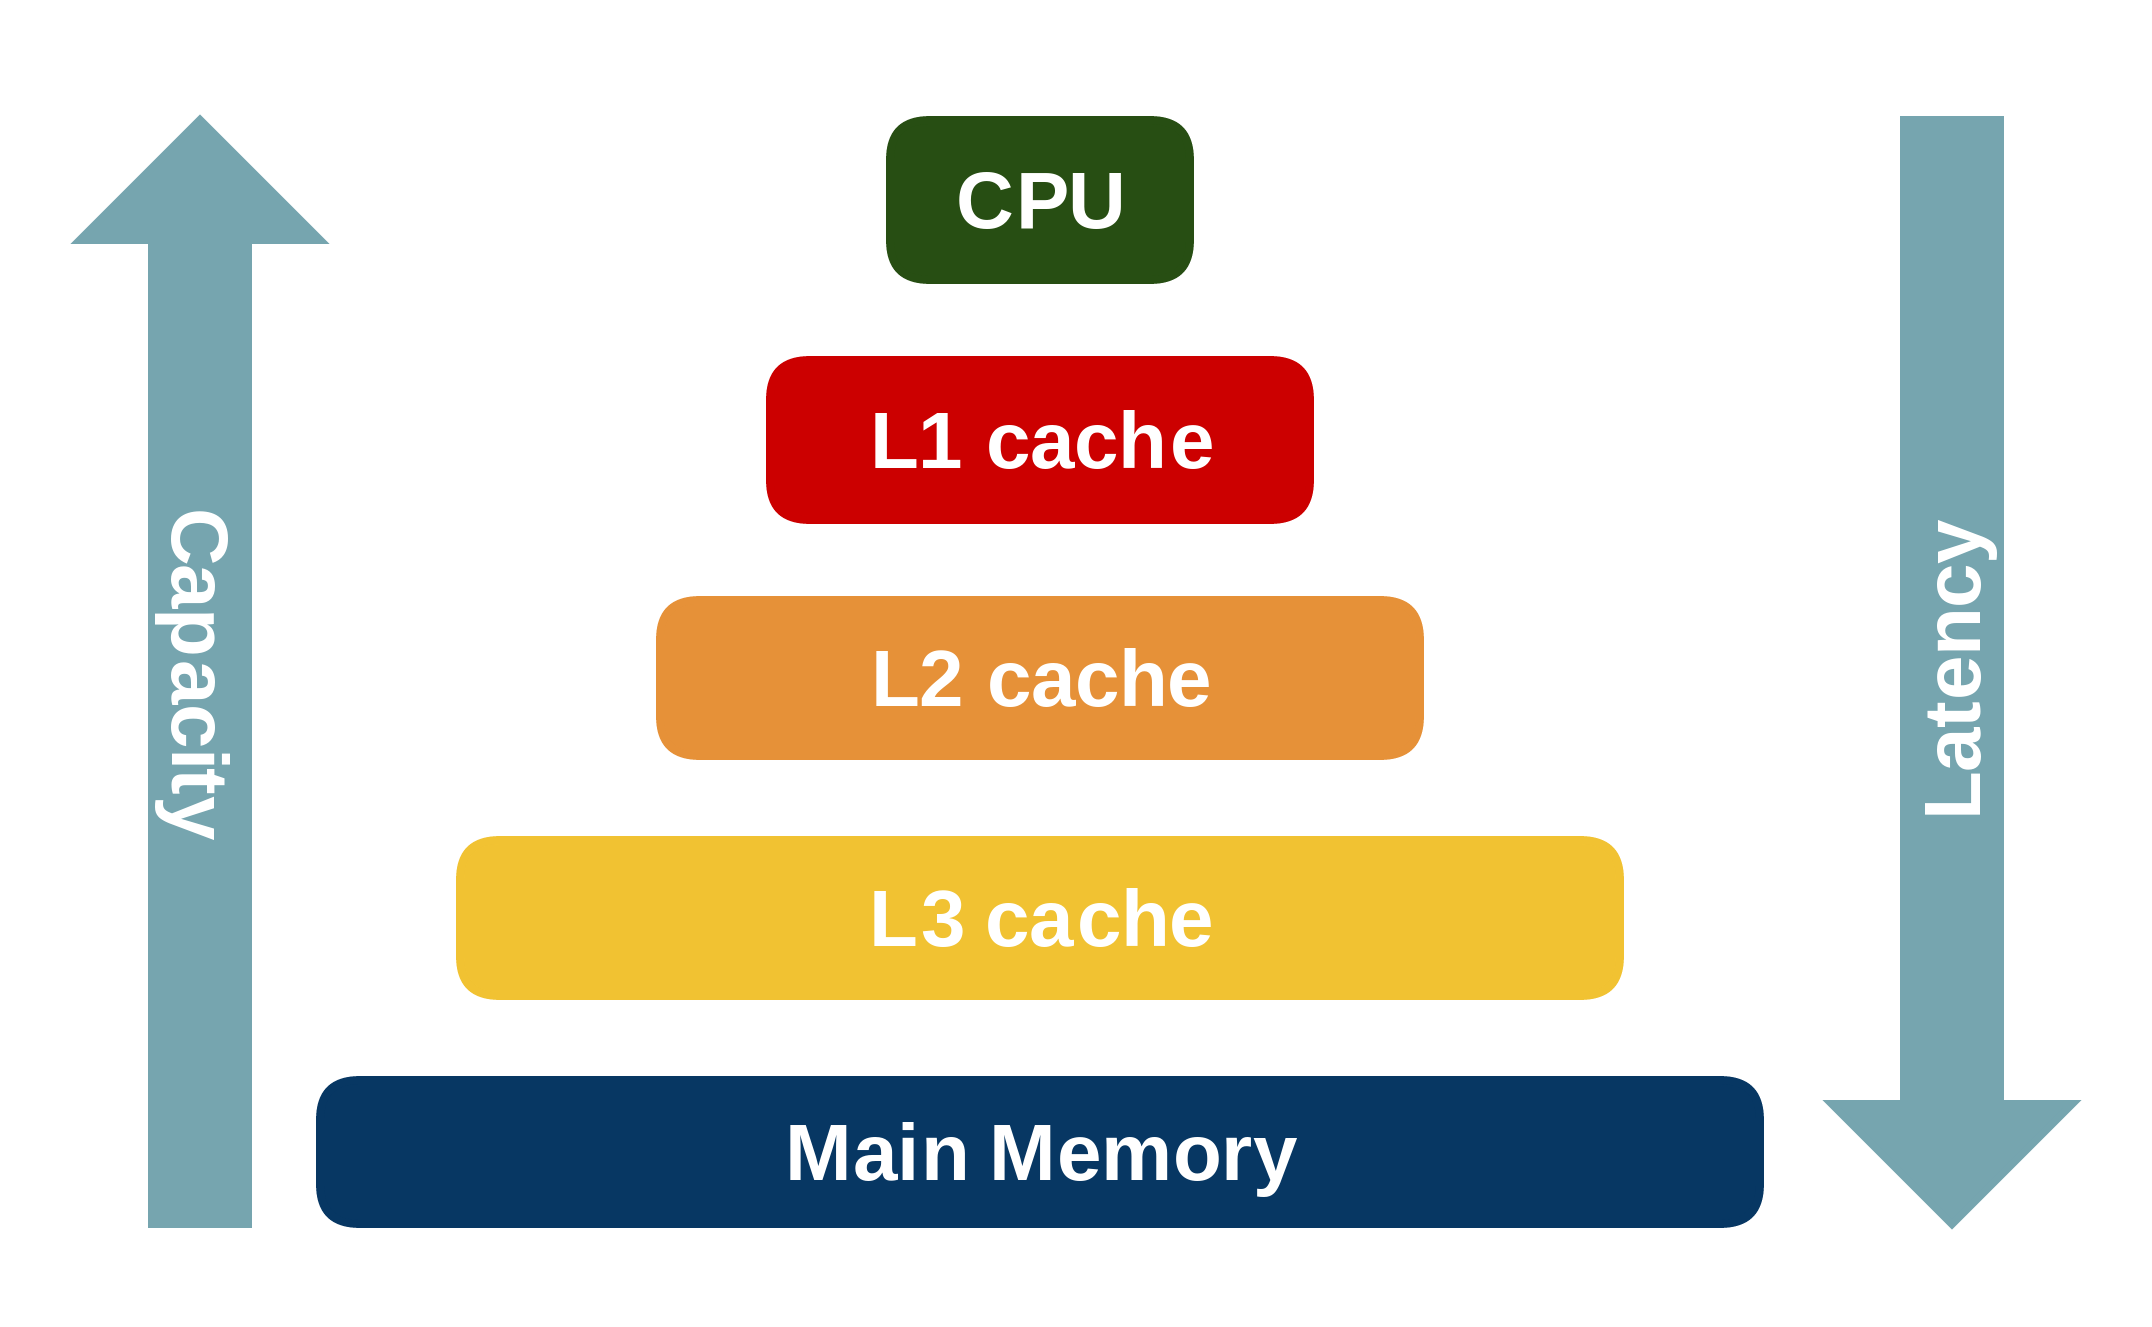
\includegraphics[height=4.5cm]{figures/cache.png}
\caption{Cache Structure\cite{cachehierarchyimg}}
\label{fig:cache}
\end{figure}

Cache memory increases the overall speed of the system by granting fast access to frequently accessed resources from the main memory. Since the size of the cache memory is generally orders of magnitude smaller than the main memory, an algorithm is used to determine the mapping of the main memory into cache and what element has to be evicted when the cache becomes full. This algorithm varies from one architecture to another and is known to change between processor generations \cite{oren2015spy}. 

The structure of the cache memory follows a hierarchical scheme. The top level contains the level 1 (L1) cache which is the smallest, fastest and closest to the CPU. The L1 cache is followed by a series of progressively larger and slower memory elements until it reaches the main memory. Typically the cache is split into three levels: L1, L2 and L3, as it can be seen in Figure \ref{fig:cache}. The cache level closest to the RAM is known as last-level cache or LLC \cite{oren2015spy}.

Multi-level caches split into two categories: inclusive and exclusive cache. Inclusive caches require that lower levels of the cache include all the data which can be found in the upper levels. Exclusive caches guarantee that data can be found in at most one cache level. The two designs have various advantages and disadvantages. Exclusive caches allow more data to be stored, while removing data from inclusive caches is generally faster since it only needs to be removed from the last-level cache. Intel's cache architecture is inclusive while AMD's cache architecture is exclusive \cite{oren2015spy}.

When the CPU needs to access physical memory it will first look for the respective address in the cache. If the resource does not reside in the cache memory, it will have to be retrieved from the main memory. This is known as a \textit{cache miss}. A \textit{cache hit} occurs when the address the CPU is looking for is found in any of the cache memory levels \cite{oren2015spy}.

\subsubsection{Cache Organization}
Since cache memory is generally smaller than main memory, various techniques are used to map main memory to cache. Main memory is split into \textit{cache pages}, a \textit{cache page} is a block of main memory which size is dependent on the cache memory. Each \textit{cache page} is further divided into \textit{cache lines}. Based on the mapping mode caches can be split into: direct mapped, n-way set associative and fully associative cache.
\begin{itemize}
\item Direct Mapped: Direct Mapped Cache is also known as 1-way set associative cache. In direct mapped mode, the main memory is divided into \textit{cache pages} equal to the size of the cache. Each \textit{cache line} can only reside in one position in the cache memory. 
\item Fully Associative: Fully Associative Cache allows any \textit{cache line} from the main memory to reside anywhere in the cache memory. In a fully associative scheme, the main memory is only divided into \textit{cache lines} and pages are completely ignored.
\item N-way Set Associative Cache: A Set Associative Cache scheme is a combination of the previous two schemes and the most common technique to map CPU caches. The cache memory is split into n equal blocks known as \textit{cache ways}. The main memory is split into \textit{cache pages} of size equal to the \textit{cache way}. Each \textit{cache way} acts like a small direct mapped cache. Each \textit{cache line} can now be stored in n positions in the cache memory. This decreased the need to overwrite the data in the cache memory.
\end{itemize}

\subsubsection{Intel's Last-Level Cache Structure}
Intel's cache architecture is inclusive, so the last level cache contains all the elements stored in the cache memory. The LLC is divided into slices one for each core of the CPU. Each core is directly connected to a \textit{cache slice}, but it also has access to all the other slices \cite{oren2015spy}.

The size of the LLC varies between processor models and ranges between 3MiB to over 20MiB. Due to its relatively large size it is not efficient to iterate through the whole cache when looking for a specific address. The LLC is further divided into \textit{cache sets}, each block of main memory maps to a specific set in the cache memory. Each \textit{cache set} contains several \textit{cache lines} \cite{oren2015spy}. 

The Intel Core i7-4960HQ processor is multi-core 4th generation Intel Core processor. The cache memory for this processor has a Smart Cache architecture. Smart Cache is an architecture developed by Intel that allows multi-core processors to share the same last level cache memory instead of having dedicated per-core cache. The processor has 8192 ($2^{13}$) cache sets, each set being 12-way associative. Every cache set can hold 12 lines of  64 ($2^6$) bytes each. The total cache size of the Intel Core i7-4960HQ processor is 8192x12x64=6MB \cite{oren2015spy}.

In a 12-way associative cache each cache line can only be stored in 12 positions in the cache memory. The algorithm that determines the mapping between a physical address and an index in cache memory is not public and has changed between processor generations \cite{oren2015spy}. Hund et el. \cite{hund2013practical} were able to reverse engineer the mapping in the case of Sandy Bridge processors.

\section{Browser Attacks}
\label{tb:browserattacks}
Traditionally, web browsers were software applications which allow users to view and interact with content on a web page. The expansion of the Internet determined browser vendors to add new features to their software. The transition from static to dynamic web pages, not only brought richer, more interactive and responsive web applications but also opened the way for a new series of attacks, known as browser attacks. The most popular attacks amongst web applications are by far cross-site scripting (XSS) and Structured Query Language (SQL) injection. Over the last few years, however, there has been an increase in attacks of web applications targeting side channel information such as the time it takes to load an external resource.

\subsection{Attack Vectors}
One of the oldest and most popular browser attacks is the disclosure of pages the user has previously visited. The majority of browsers change the color of a link if the user has visited it before. The change can easily be done using the CSS:visited pseudo-class. An attacker can request the computed style using JavaScript and therefore gain access to the victim's browser history \cite{cssvisited}. Researchers discovered that this techniques was being used by numerous high-profile websites to obtain a user's browsing history
\cite{jang2010empirical}.

Analysing the style of a web page is not the only way to expose a user's browsing history. A similar attack, discovered by Felten et al. \cite{felten2000timing}, uses timing information to determine if a web page has been previously visited by the victim. This attack assumes that recently accessed resources will be cached by the browser in order to provide faster loading times during future visits. By comparing the loading time of different web pages an attacker can determine if a file is in the user’s cache, and hence whether or not the user has accessed that website before.

Websites customize their services according to the users’ locations. For example, a user accessing Google from within the United Kingdom will be redirected to www.google.co.uk. Jia et al. \cite{jia2015know} have shown that is possible to derive a user's location by simply checking what local version of the website is stored in their browser's cache memory.

Another class of browser attacks was identified by Bortz et al. in \cite{bortz2007exposing}. If previous attacks were targeting static resources, which can be cached, their attack is aimed at dynamically generated web pages. Bortz et al. \cite{bortz2007exposing} present two types of attacks: \textit{direct timing} attacks, where an adversary has direct access to a website and is able to obtain information about the website's state by simply measuring the server's response time, and \textit{cross-site timing} attacks, where an adversary tries to obtain information about the victim's view of a cross-origin website.

The measurements techniques used by Bortz et al. \cite{bortz2007exposing} are dependent on network conditions and could provide erroneous results. Van Goethem et al.\cite{van2015clock} extended the work of Bortz et al. \cite{bortz2007exposing} and presented new timing methods, which are independent of the victim's network condition, thus provide more accurate timing information. 

Oren et al. \cite{oren2015spy} identified a new category of side-channel attack which run in the browser. The work described in \cite{oren2015spy} uses the state of the browser's cache memory to determine what web site the victim is currently visiting.

\subsection{Web Browsers}

A web browser is a software used for interacting with web applications. The main functions of web browsers are retrieving the requested resource and displaying it in the browser window. In order to display the web document, browsers use rendering engines. There are multiple rendering engines available and different browsers use different engines. According to \cite{statcounter} the top 3 most popular browsers among desktop and tablet users are Chrome (56\%), Firefox(14\%) and Internet Explorer(12\%). They all use different rendering engines, Chrome uses Blink, Firefox uses Gecko while IE uses Trident\cite{howbrowserswork}.

Rendering engines parse the HTML documents and create an output tree made out of Document Object Model (DOM) nodes. The rendering engine is also responsible for gathering all the style information about the DOM nodes. The final output of the engine is the render tree which is ready to be displayed by the browser\cite{howbrowserswork}.

The DOM is a programming interface which allows a more versatile way of accessing the HTML document. It can be easily manipulated by scripting or programming languages in order to change the structure, style or content of the original document\cite{dom}.

\subsection{HTML}
HyperText Markup Language, known as HTML, is a markup language used to create web pages. Initially designed as a language for semantically describing scientific documents, HTML became the standard markup language for building web documents. HTML is used to describe the structure and semantic content of a web page, but not its functionality\cite{world1999html}.

HTML consists of a set of elements, which define the structure of web pages. Most HTML elements are composed of a start tag, \texttt{<element>}, and an end tag, \texttt{</element>} ,with the content nested in between the two tags. The end tag is optional and all browsers will display documents which do not contain a matching closing tag for each opened tag; however, this technique can produce unexpected results and it is not recommended. Furthermore, strict HTML document validators require that elements have both a start and an end tag\cite{world1999html}.

HTML also includes a number of empty elements, elements formed of only a start tag or a start tag with the backslash appended to the element name, \texttt{<element/>}, with no content, such as \texttt{<br>}, which defines a line break. The HTML standard does not specify which of the two ways of representing an empty element is preferred. Though, the latter provides stricter validation and is accepted by XML parsers\cite{world1999html}.

HTML elements can have attributes. Attributes are (key, value) pairs which determine the behaviour of elements, such as \texttt{color}, \texttt{font} or \texttt{position}. Attributes must be specified in the element's start tag\cite{world1999html}.

HTML5 is the 5th and current version of the HTML standard. It was released in 2014 by the World Wide Web Consortium (W3C). The current version of HTML introduced a number of new features aimed at simplifying the incorporation of multimedia and graphical content into web based applications\cite{berjon2014html} such as the Audio and Video elements.

\subsubsection{Media Elements}
HTML elements are the basic building blocks of web pages. Apart from providing the overall structure of the web page, some HTML elements are used to embed media into a web page. HTML has always provided support for embedding media into web pages and newer versions of the language further simplify the process by introducing elements aimed exactly at this. The \texttt{<img>} element, available sine HTML 4.1, allows the insertion of images while the \texttt{<audio>} and \texttt{<video>} elements introduced in HTML5 enable audio and video content incorporation into web applications.

\paragraph{Image}
The \texttt{<img>} tag is used to represent an image in a HTML document. The address to the resource to be displayed is stored in the \texttt{src} attribute. In order to successfully embed an image in a web page, the \texttt{src} attribute has to be present and it must contain a valid non-empty URL\cite{berjon2014html}.

The browser starts by downloading the external resource from the address provided in the \texttt{src} attribute or an alternative address if this is not available. The \texttt{<image>} element has a series of events associated with it, which fire at various times. One such event is the \texttt{load} event, which announces that the browser has finished downloading the resource and is ready to display it. 
Occasionally, the browser is unable to display the file as an image, due to the resource not being a valid image file or other error which might have happened during the download process. In these cases, the \textbf{error} event will be triggered in the Image object once the browser becomes aware that something went wrong \cite{berjon2014html}.

The browser is unable to identify if the URL stored in the \texttt{src} attribute is a valid image file until it has downloaded the resource. The \texttt{error} event will fire once the file has been downloaded. The total download time of the file is dependent on the resource's size and the speed and stability of the network connection. The time elapsed since the \texttt{src} attribute was set until the \texttt{error} event is triggered on the element grows with the size of the external resource.

\paragraph{Video and Audio}
The \texttt{<video>} and \texttt{<audio>} elements were introduced in HTML5 and enable web developers to easily embed audio and video content into their applications. The most recent version of HTML makes the insertion of a video into a web application as easy as adding an image \cite{berjon2014html}.

Similarly to the \texttt{<img>} element, files loaded as a \texttt{Video} or \texttt{Audio} element need to be downloaded before the browser can decide if they are valid video or audio files. Additionally, in some browsers, such as Chrome, the browser needs to parse the contents of the file before it can determine if the resource can be played. This is not the case of Firefox, where the \texttt{error} event will fire as soon as the resource has finished downloading and the browser tries to read its contents. The \texttt{video} and \texttt{audio} elements have additional events associated with them. Apart from the usual, \texttt{error} and \texttt{load} events, the browser is able to tell if the resource loaded as a video is still downloading by firing the \texttt{progress} event or if the resource has finished downloading by triggering the \texttt{suspend} event. 

In order to display a media file, the browser will start by downloading the external resource. While the file is being downloaded the \texttt{progress} event is being triggered. When the file has been fetched or if the downloading process has been paused the \texttt{suspend} event is fired. The browser proceeds by parsing the contents of the file in order to obtain information such as the length, width, height or extension, etc. of the file. If the media resource is not a valid file the browser will not be able to display it and the \texttt{error} event will be triggered on the media element. The time elapsed between the \texttt{suspend} and the \texttt{error} events is depended on the size of the file. The \texttt{error} event fires on the media element when the browser has finished parsing the file in contrast to the \texttt{Image} element, where the event is triggered when the browser learns that the file is not valid, usually as soon as it starts parsing it\cite{berjon2014html}.

\subsection{JavaScript}
\label{javascript}
JavaScript is an interpreted scripting language generally used on the client side of web applications. Developed independently by both Netscape and Microsoft, it has been standardized by ECMA International under the name ECMAScript. The most recent version is ECMAScript 2017. ECMAScript, and thus JavaScript is supported in all modern browsers. JavaScript is the most widely used client side language \cite{javascriptstats, javascriptabout}.

JavaScript's main role is to add dynamic behaviour to web applications through modifying the DOM. The use of technologies to make dynamic and animated web pages is known as Dynamic HyperText Markup, DHTML. DHTML allows scripting languages such as JavaScript to make changes to the DOM in order to alter the appearance or function of the static HTML elements.

To add JavaScript to an HTML document the special \texttt{<script>} HTML element is used. JavaScript code can either be embedded in the page or it can be loaded from an external file. Keeping HTML and JavaScript separate is the preferred choice as it helps with both performance and maintenance.

For security reasons, JavaScript has severely restricted access to the system. JavaScript needs the user's explicit permission in order to access system files, even for reading. JavaScript has no notion of pointers and does not support direct memory access. Despite these drawback, there are numerous Application Program Interfaces (APIs) available which provide additional features.

\subsubsection{Typed Arrays}
\label{typedarray}

JavaScript supports Array, which are used to store multiple elements into a single variable. JavaScript Arrays are dynamically resizeable and can hold anything from objects to another array. One disadvantage of native JavaScript Arrays is that the containing elements do no necessary reside in sequential blocks of memory. This can bring severe performance penalties when sending data to external APIs, such as WebGL \cite{webgl}.

JavaScript Typed Arrays \cite{typedarrays} are a relatively new API born from the need to access raw binary data, which is not possible in plain JavaScript. Typed Arrays allow the allocation of a fixed sized buffer of binary data in memory. The advantage of using Typed Arrays is that the buffer can be efficiently passed to native libraries, which require access to binary data.

Compared to the C programming language, JavaScript does not support the declaration of fixed sized arrays. For example, it is impossible to declare an array of 4MB in JavaScript. The Typed Arrays API can be use to solve this issue.

\subsubsection{High Resolution Time API}

User experience in modern web applications is greatly influenced by the application's performance. As web applications get more and more complex, analysing its performance becomes a key issue. Existing timing APIs provide millisecond time measurements; however, this lacks the precision needed for good understanding of the underlying problem. The JavaScript High Resolution Time API contains one method, \texttt{performance.now}, which returns the number of microseconds elapsed since the page has started loading. 

The JavaScript High Resolution Time API \cite{jshighresolutiontimeapi} provides time measurements accurate to a microsecond. Previous versions of the API used to provide submicrosecond time measurements. Due to security issues, the API had to be changed and it no longer provides such accurate time measurements. Recent versions of Firefox and Chrome restrict the time measurement even further by classifying as 0 all time measurements less than 5 microseconds.

\subsection{Offline Experience}
Web applications are dependent on network availability and cannot function if there is no network connection or in most cases even if the network connection is unstable or not strong enough. Web applications fall into two categories: those that provide access to data: YouTube, Wikipedia or Twitter and those that let users do stuff: Google Keep, Google Docs or CSS Lint.

The first category has access to large amounts of data, but users only use a small portion of it at a given time. One of the ways such applications can be improved is by retrieving the data faster, which relies mostly on the network provider and not the application developer. The second category of applications handles a small amount of data and most of the computation happens on the client's device. 	The application data rarely changes and it would be a waste of network resources to retrieve the data every time it is used. 

One solution to avoid these needless overuse of the network would be to store some of the data locally. At its simplest an offline web application would have all the needed resources stored locally and when there is no network connection the application would fetch the local copy of the file instead of the remote one.  Web developers have started to provide offline access to their applications for some time and there are several methods to achieve this.

The most basic way of storing data is in the browser's cache memory. All browsers are capable of storing web pages if told to do so; however the web developer has no control over the browser's cache. It is up to the browser to decide what pages to keep and what pages to remove from the cache when it becomes full. 

\subsubsection{Application Cache}
\label{applicationcachetb}
Application Cache \cite{appcache} or AppCache is a framework which provides caching of resources in order to be later accessed offline. The AppCache API is part of HTML5 and allows web developers to specify which web pages and resources should be cached by the browser and made available offline.

AppCache provides two ways to cache resources: either by specifying the path to the resource in the cache manifest or by including the cache manifest in the header of the document to be cached. The cache manifest is a text file containing the addresses of all web pages that should be stored locally. Despite being easy to use, AppCache does not allow developers to make any changes to its system. 

Although it solves one of the main issues faced by web application developers, offline access, AppCache has a number of disadvantages. Once a resource is cached it will always be fetched from local storage even if the network conditions are good. AppCache does not provide easy update of currently cached resources and is unable to identify any changes made to the remote file. The only way to update the resources cached locally is either to empty the cache or make changes to the manifest file.

All this drawbacks determined developers to move away from AppCache and work towards developing new software for improving users' offline experience. Despite major browsers providing software for interacting with the Application Cache mechanism, they are currently removing support for this framework.

\subsubsection{Web Workers}
JavaScript is a single-threaded scripting language. Web applications developed using JavaScript have a main UI thread responsible for DOM access and sequentially running the scripts loaded in the HTML documents. If multiple scripts are loaded on the same page, JavaScript will wait for the previous scripts to finish before starting the next one. Long JavaScript tasks would make the application unresponsive so this created a need for multi-threading in JavaScript. One way to achieve multi-threaded behaviour in JavaScript is through web workers. Web workers are background JavaScript scripts that run in parallel to the main application. Web workers do not have DOM access; however, they can communicate with each other and the main UI thread.

\subsubsection{Service Workers}
Application Cache was one of the first frameworks whose main role was to provide offline experience in web based applications. Web application developers have to tailor their product to meet the needs of the AppCache mechanism instead of make changes to AppCache to fit the needs of the product. This problem was fixed by Service Workers which allow developers more freedom when determining the offline behaviour of their application.

Service Workers are event driven web workers which sit between the network layer and the application layer. Service Workers were inspired by AppCache, their main purpose is still proving users with the offline experience. What makes Service Workers different is that they give developers complete control over what the offline experience will be. 

Compared to AppCache, Service Workers do not store the data needed to run the application in offline mode. Service Workers monitor the network and are able to over-ride default network behaviour. They communicate with other services such as the Cache API that deals with the actual storage part. Typically, a Service Worker would monitor requests sent by the application and either serve the data from local storage if available or fetch it over the network and save it locally for later retrieval. 

The Cache API stores (key, value) pairs where the key is the URL and the value is the response returned by fetch. The Cache API ignores the \texttt{"no-cache"} and \texttt{"no-store"} HTTP header. Resources which contain the \texttt{"no-cache"} or \texttt{"no-store"} HTTP header can still be cached, however they cannot be displayed. 

Service Workers are registered against an origin and a path and requests made from this location will trigger the service worker events. The events will not only fire for every page request within the Service Worker's scope but also for requests made by those pages. Service Workers allow CORS (Cross-Origin Resource Sharing) - requesting a page from a domain outside the domain from which the page originated.

Service Workers run independent of the application they are monitoring. Service Workers need to be linked to the application once it is running and can only monitor applications which started while it was active. The first time the application is started the Service Worker will be linked to the application and start running. Once the Service Worker script is working, the application needs to be restarted, such that the Service Worker can start collecting network information about the application. If the Service Worker is active it can only be closed by stopping the script from the browser, the main application has no control over the Service Worker.

At the moment Service Workers are fully supported in Chrome and Firefox for both desktop and mobile and have basic support in Opera. Microsoft newest browser, Edge, is also working on adding support for this new technology.


%%%%%%%%%%%%%%%%%%%%%%%%%%%%%%%%%%%%%%%%%%%%%%%%%%%%%%%%%%%%%%%%%%%%%%%%%%%%%%%%%%%%%%%%%%%%%%%%%%%%%%%%%%%%%%%%%%%%%%%%%%%

\chapter{A Preliminary Analysis of Published Attack Vectors}
\label{chap:realtedWork}

In this chapter I am going to review some of the most important browser attacks, analyse their effectiveness and determine if they are still possible. Section \ref{feltenschneider} describes on of the oldest browser attack, which reveals if a given resource is being fetched over the network or from the browser's cache memory. Another type of browser attacks, outlined in Section \ref{cssatt}, targets a vulnerability in the browser software which grants an attacker access to what links a user's has visited. The attack presented in Section \ref{location} allows the disclosure of a user's location. Bortz et al.\cite{bortz2007exposing} were the first to attack dynamically generated HTML pages and disclose the amount of hidden data a user has access to, the results of their attack are presented in Section \ref{bortz}. In Section \ref{van} I describe a series of novel measuring techniques proposed by Van Goethem et al.\cite{van2015clock}, which can be used to determine the size of a cross-origin file. Section \ref{orenetal} presents a browser cache timing attack, which reveals the user's browsing activity.

I chose the six attack because they target the disclosure of different private information about users: from location to what websites they are currently browsing and the amount of data they have access to on various social media websites. In the rest of this chapter I am going to look at why are these attacks possible and if the proposed countermeasures were efficient in stopping the attacks.

\section{Felten and Schneider - Timing Attacks on Web Privacy}
\label{feltenschneider}
Felten and Schneider were the first to identify a vulnerability in the browser's cache mechanism which lets an adversary spy on a user's browsing history. The attack, which uses timing information to determine if a web page has been previously visited by the victim, is described in their 2000 paper \cite{felten2000timing}.

Their attack model assumes that the victim accesses a web page containing attacker-controlled content. For example, an attacker Eve wants to see if the victim, Alice, has recently been to Bob's website. Eve builds a malicious website which sends a request to Bob's web page and measures the time it takes to receive the response. When Alice accesses Eve's website, the spy process automatically computes the time it takes to access Bob's website and sends the result to Eve. If the time is less than some threshold, Eve concludes that Bob's web page is stored in Alice's cache, therefore Alice has recently accessed Bob's web page. On the other hand, if the time to access Bob's web site is greater than the threshold, Eve learns that Alice has not been to Bob's web site.

Felten and Schneider outline several methods for convincing the victim to access the malicious web page, such as \cite{felten2000timing}:
\begin{itemize}
\item Embedding the attack into the web site of a well known organization that wished to spy on its customers, such as a health insurance company that wants to know if the user has recently accessed web pages about a particular medical condition.
% https://searchenginewatch.com/sew/study/2215868/53-of-organic-search-clicks-go-to-first-link-study
\item Adding the attack content to a website that ranks high in search results. 
\item Assuming the victim uses an HTML-enabled mail reader, the attacker could send an email with an HTML message body containing the malicious code.
\item The attacker could send the victim an email with a message that will convince the victim to access the attacker's website. This techniques is similar to phishing emails, where the goal is to gain access to a user's credentials.
\end{itemize}

The attack can be easily implemented in Java or JavaScript. Felten and Schneider also provide an alternative method for measuring the time using HTTP requests when Java and JavaScript support is turned off. They also analyse different methods for determining the threshold value based on how much information the attacker has about the victim's system.

Felten and Schneider discuss several countermeasures for this attack and analyse their efficiency in real world scenarios. The first solution they suggest is the use of the \texttt{"no-store"} and \texttt{"no-cache"} HTTP headers \cite{felten2000timing}. This prevents the files from being stored in the browser's cache memory, so an attacker would be unable to determine if the victim has accessed the web page before. One major drawback of the cache control headers is that they do not stop resources referenced by the page from being cached. For example, if a web page containing an image has the \texttt{"no-store"} and \texttt{"no-cache"} HTTP headers attached, the browser would still cache the image file, thus allowing an attacker to distinguish between a visited web page and a web page which the user has not accessed.

Another class of countermeasures suggested by Felten and Schneider is turning off some of the browsers features such as caching or Java and JavaScript \cite{felten2000timing}. Disabling caching would prevent the attack; however, it will bring major performance penalties since browsers rely on caching to deliver content faster. The researchers already provide an alternative for measuring the time on the server side through HTTP call when Java and JavaScript are not enabled, so disabling them would not prevent an attacker from learning about the victim's browsing history.

The use of VPN software is briefly mentioned as a measure to prevent the attacker from spying on the victim. Unfortunately, this adjustment makes the attack easier as the added delay amplifies the time difference between hits and misses, thus making the two distributions distinguishable. 

The final countermeasure mentioned in the paper is altering hit or miss performance in an attempt to make them indistinguishable. Felten and Schneider claim that this change does not affect the performance of their attack. For the two distributions to be indistinguishable, hits should be as slow as misses which would make caching useless and decrease the browser's performance. Otherwise, hits will always be faster than misses, therefore an attacker could differentiate between the two cases \cite{felten2000timing}. 

Felten and Schneider also discuss the possibility of changing the browser's cache implementation in order to prevent some timing attacks \cite{felten2000timing}. They propose adding the domain as an attribute to every element stored in the browser's cache and only allowing access to pages which share the same domain. For example, if the page www.searchengine.com contains the media element image.gif, image.gif will be stored in cache with the domain set to \textit{searchengine}. When www.adversary.com tries to access image.gif, the resource will be fetched from the server and not from the browser's cache because the domains of the requester, \textit{adversary}, and the resource, \textit{searchengine}, do not match. It is hard to measure the efficiency of this solution since it requires changing the browser software. In December 2000, Princeton University announced that Felten was working on implementing domain tagging; however, nothing has been released since \cite{princetonunifelten}.

Although the attack was discovered over 15 years ago, no one has been able to come up with a solution that will both maintain a browser's caching capabilities and protect the user's privacy. 

\section{CSS Attack}
\label{cssatt}

In 2002, Clover discovered a feature in CSS that would leak what pages a victim has previously visited \cite{cssvisited}. The attack achieves similar results as the the one proposed by Felten and Schneider in \cite{felten2000timing}; however, the feature identified in CSS ``is simpler, more accurate, and more easily abused" as Clover describes it in \cite{cssvisited}.

The majority of browsers change the color of a visited link such that a user can tell what linked they have already accessed. The change can easily be done by using the CSS:\texttt{visited} pseudo-class. An attacker can request the computed style using JavaScript and therefore gain access to the victim's browsers history \cite{cssvisited}.

Clover proposed three possible solutions and analysed their likelihood of solving this issues. His first suggestion is to send the visited style regardless of the state of the link, visited or not. Although, this would stop attackers from distinguishing between the two types of links when requesting the computed style, some browsers offer additional software that would still make the attack possible. He also recommended that users be advised to turn off scripting when visiting untrusted pages. His last suggestion is the use of domain tagging, introduced by Felten and Schneider in \cite{felten2000timing} and explained in Section \ref{feltenschneider}.

Clover stated that none of the proposed solutions is a valid countermeasure. He also thinks that the attack is possible due to a CSS implementation issue rather than being a browser related problem \cite{cssvisited}. It is unclear if the attack discovered by Clover is still possible. 

In 2010, Baron, a developer from Mozilla Corporation, presented a method which he claims can stop Clover's attack and announced that Mozilla was planning to include the countermeasure in the new release of the Firefox browser \cite{fixedcssprivacy}. Baron's solution is to change the browser's implementation of the function which requests the computed style such that it sees all URLs as unvisited. When an adversary asks for the computed style, they will be unable to distinguish visited URLs from unvisited ones. Additionally, Baron suggests allowing users to opt out of using the feature which changes the colour of visited links. He agrees, however, that this would not completely stop the attack, since developers can use other techniques to differentiate between visited and unvisited URLs, such as adding a background image to visited links or increasing the font size of visited URLs.

\section{Jia et al. - I Know Where You've Been: Geo-Inference Attacks via the Browser Cache}
\label{location}
Traditionally a user's location could by determined by checking their IP address; however, multiple studies showed that this can give imprecise results. Users can use anonymization services such as VPNs and the Tor \cite{tor} browser in order to hide their real IP addresses, making the IP address useless when determining their real location. The recent increase in popularity of mobile devices brought new methods of detecting a user's location such as GPS sensors. By default, access to GPS data is turned off and requires a user's explicit permission. 

Geo-location information is treasured by websites which provide location-specific services as it enables a more personalized experience for users. For example, a user accessing Google from within the United Kingdom will be redirected to \textit{www.google.co.uk}. One the other hand, attackers are also interested in obtaining a user's location for various reasons from social engineering attacks to targeted advertisements. Jia et al. \cite{jia2015know} show how it is possible to infer a user's location using side channel information from the browser's cache. They analyse the efficiency of several methods for obtaining a user's geo-location and present different countermeasures and their likelihood of defending against this attack in their paper \cite{jia2015know}.

Jia et al.'s \cite{jia2015know} attack is based on the assumption that users generally visit location-oriented websites for the locations that they currently live in or plan to visit. Additionally, a large number of websites provide information for local residents, thus, the majority of people who access those web pages live in the area. 

The requirements for running the attack are minimal. An attacker needs to have access to a server and a website running JavaScript that has to be accessed by the victim. Once the victim navigates to the attacker-controlled web page, the background script starts the process of determining a user's geo-location. The attack model assumes that an attacker is able to distinguish between a cache hit and a cache miss and that recently accessed resources are cached, hence the victim does not regularly clean their browser's cache memory.

Jia et al. \cite{jia2015know} successfully determined a user's country, city and even neighbourhood using different measurement techniques. They showed that the attack affects all mainstream browsers including Tor. Additionally, they determined that over 60\% of Alexa Top 100 \cite{alexa500} websites provide location-specific content, therefore they are vulnerable to geo-inference attacks \cite{jia2015know}.

Google has 191 location-specific domains used to provide personalized search results. Additionally, Google uses a different logo for each of these websites. The researches were able to determine a user's location by simply checking which of the 191 logos was served from the browser's cache memory. In order to obtain the measurements, they requested each logo three times. If the logo was being retrieved from cache there would be almost no difference between the three values. On the other hand, if the image was fetched over the network there would be a significant difference in time between the first request and subsequent requests \cite{jia2015know}.

Jia et al. \cite{jia2015know} were able to determine a user's city and neighbourhood using similar measuring techniques. For obtaining a user's city, they made use of Craiglist \cite{craiglist}, which offers different websites for 712 cities around the world. The researchers discovered and exploited the fact that Google Maps is a collection of map tiles each with a unique URL, containing geographical coordinates \cite{jia2015know}. Although they proved that determining a user's neighbourhood is possible, the attack might be impractical since it requires analysing large data sets. They estimate that for the city of New York it takes around 8 minutes to detect a user's neighbourhood. \cite{jia2015know}.

The paper also presents the advantages of disadvantages of potential countermeasures. Jia et el. \cite{jia2015know} justify that private browsing, the use of anonymization software or randomizing timing measurements do not affect the attack. They suggest that websites should provide a non-geo-targeting version of their website which users can opt to use. The last solution they propose is browser cache segregation, this prevents cross-origin websites from accessing resources cached by the original web site. Although, similar solutions have been proposed before to solve various side channel attack which affect browsers, none of the browser vendors have implemented this solution as it is believed to bring significant performance overhead. They conclude by saying that the same-origin policy on the browser cache is the best available solution and argue that the performance overhead can be reduced \cite{jia2015know}.

The attack presented by Jia et al. \cite{jia2015know} was discovered over a year ago; however, the researchers are exploiting vulnerabilities which have been around for over a decade. The first such attack, discovered by Felten and Schneider \cite{felten2000timing}, is described in Section \ref{feltenschneider}. By far, the most common countermeasure proposed in all the papers, which exploit similar vulnerabilities, is the use of the same-origin policy on the browser's cache memory. Jia et al. \cite{jia2015know} even implemented this feature on an open source browser. It is unclear why browser vendors refuse to add this feature to their software. 

Despite the same-origin policy on the browser's cache memory being proposed as a countermeasure against browser cache timing attacks by numerous researchers, it is yet to be implemented in modern browser software. I believe one of the main reasons why browser vendors refuse to add this feature to their software is because it might reduce the browser's performance. Jia et al.\cite{jia2015know} claim that the performance overhead can be reduced; however, they do not provide any physical evidence.

\section{Bortz et al. - Exposing Private Information by Timing Web Application}
\label{bortz}
Another class of browser attacks was identified by Bortz et al. in \cite{bortz2007exposing}, where they use the time that servers take to respond to HTTP request as a side channel. The paper presents two types of attacks: \textit{direct timing}, where the attacker has direct access to a website, and \textit{cross-site timing}, where the adversary uses the victim's view of the website to obtain private information. The researchers tested their attacks on two real world scenarios: obtaining the value of some boolean condition and estimating the size of hidden data \cite{bortz2007exposing}.

In \textit{direct timing} attacks, the adversary has to access a website and use the timing information obtained to infer certain properties about the secret data. The easiest attack would be a boolean test, where the adversary tests if some condition on the server's hidden data holds or not. For example, the majority of web sites, which require a username and password for log in, have a forgot my password page. The adversary could use that page to obtain a list of valid email addresses as the victim websites usually display an error if the email address is not in their data base. There are known countermeasures against this type of attack such as: limiting the number of tries or requesting additional information; however, there are still websites vulnerable to this simple attack \cite{bortz2007exposing}. 

\begin{lstlisting}[caption={Example JavaScript timing code as shown in \cite{bortz2007exposing}},label={bortz}, language=HTML, showstringspaces=false]
<html><body><img id="test" style="display: none">
<script>
	var test = document.getElementById('test);
	var start = new Date();
	test.onerror = function() {
		var end = new Date();
		alert("Total time: " + (end - start));
	}
	test.src = "http://www.example.com/page.html";
</script>
</body></html>
\end{lstlisting}

Direct timing attacks can also be used to estimate the size of hidden data. The paper gives several examples of web applications vulnerable to this type of attack, such as Gallery\cite{gallery} a photo album organizer. The application allowed users to upload photos and choose if they want to make them public or private. Public means that everyone has access to the photos, while private photos are only accessible by the album's owner. An attacker accessing the album would only see the public photos; however, they could determine the total number of photos in the album, public and private, using timing information. The attack was possible because the server would request all the photos in the album, and then display only the ones the requester had access to Bortz et al. \cite{bortz2007exposing} discovered that the size of the hidden data was strongly correlated to the time it takes to satisfy the request, therefore they were able to accurately determine the size of the hidden data only having access to time measurements. 

The other kind of attacks presented by Bortz et al. \cite{bortz2007exposing} in their paper are \textit{cross-site timing} attacks. In this type of attacks the adversary gains access to the victim's view of a website. For example, the attacker, Eve, wants to see Alice's view of Bob's Facebook profile page. Eve builds a website, www.eve.com, which when accessed sends a request to Bob's Facebook profile, www.facebook.com/bob. Bob's profile page is private and only visible to Bob's friends. Bob's friends are able to see his photos and wall posts, someone who is not a friend of Bob's will see an empty page. There is a difference in the amount of data received by a user who is friends with Bob and a user who is not. A web application which is able to differentiate between two files of different sizes will also be able to make an assumption about whether or not Alice and Bob are friends. When Alice accesses Eve's malicious application, the website receives Bob's profile information seen from Alice's perspective, approximates the size of the received data based on the time measurements and sends the result to Eve. If the size is less than some threshold (say, 500kB), Eve concludes that Alice and Bob are friends; otherwise, she concludes that the two do no know each other.

Bortz et al. \cite{bortz2007exposing} compare several methods of estimating the size of the hidden data. The first thing they tried was to load the response into an \texttt{FRAME} or \texttt{IFRAME} element; however, this method does not give accurate timing results. The \texttt{FRAME} and \texttt{IFRAME} load not only the data but also  all the the images, applets, scripts and stylesheets associated with the embedded page adding an unacceptable amount of noise to the timing measurement.

Browsers are unable to tell if a resource loaded into an \texttt{<img>} element is a valid image file until the file has finished downloading and they read the response's header. The time elapsed between sending the request and the error notifying that the file is not valid is used to estimate the size of the resource. Another method used by the researchers was to load the data into a \texttt{<link>} or \texttt{<script>} element. Browsers have to process this elements sequentially, so attackers can easily obtain timing information which can be used to estimate the size of hidden data \cite{bortz2007exposing}. The timing method used in the paper can be seen in Listing \ref{bortz}.

Both types of attack are influenced by noise; however they are affected in different ways. Direct timing attacks are vulnerable to varying network conditions and server load. Bortz et al. suggest taking multiple measurements and choosing the smallest one as it is the least likely to have been influenced by noise. If the network conditions can be estimated in a direct attack, an attacker is unable to tell what kind of connection a victim has in a cross-site timing attack so they need additional measurements in order to obtain accurate results. The paper suggests using two sources: one being the page containing the hidden data and the other one a page that which has almost no dependency on the hidden data, such as a web site's 404 page \cite{bortz2007exposing}. 
Since the size of the 404 page is known or can easily be determined on the attacker's machine, the adversary can compare the two measurements, the time it takes to load the hidden data and the time it takes to access the 404 page, in order to approximate the size of the hidden data.

Bortz et al. also analysed the efficiency of various countermeasures. The agree that adding random delays on the server has almost no effect in stopping the attack since an attacker would still be able to distinguish between files of different sizes. On the other hand, a server with constant time responses and removing timing functionality from JavaScript could stop the attack. Although, the second solution could stop the majority of browser attack, it is very unlikely that browser vendors will adopt the proposed changes to JavaScript. Also, the majority of timing attacks give alternative measurement techniques for when JavaScript is disabled.

The attack presented by Bortz et al. \cite{bortz2007exposing} is vulnerable to changing network conditions. Van Goethem et al. \cite{van2015clock} expand this attack and focus on detecting vulnerabilities in HTML and JavaScript that give more accurate timing measurements by removing the dependency on a victim's network  conditions. The browser timing attack described by Bortz et al. \cite{bortz2007exposing} is still possible; however, in recent years, similar attack but with better performance have been discovered. 

\section{Van Goethem et al. - The Clock is Still Ticking: Timing Attacks in the Modern Web}
\label{van}

Web-based timing attacks have been around for over a decade; however, it is very rarely that an attacker is able to obtain meaningful information on the state of the user in a cross-origin website since running the attack requires special network conditions. The increase in popularity of mobile devices means that more and more users connect to the Internet over wireless or mobile networks. These types of connections are often unstable and do not meet the necessary requirements to perform a cross-site timing attack. Van Goethem et al. claim to have found new methods to obtain measurements in a cross-site timing attacks which are not dependent on network conditions \cite{van2015clock}.

Their research builds on previous work by Bortz et al.\cite{bortz2007exposing} and presents four new measuring techniques which are not dependent on network conditions, and therefore give more accurate timing results. The timing techniques explore recently added features to web browsers and web development technologies such as HTML5 and JavaScript. Van Goethem et al. claim that the new found methods outperform previous attacks in both speed an reliability \cite{van2015clock}. Their paper describes four new measuring techniques: loading the external resource as a video file, using Application Cache, using Service Workers, and loading the external resource as a script. The four methods are described in more detail below. Then, Van Goethem et al. \cite{van2015clock} present several real world scenarios, where the attacks can be used to obtain private information about a user, and conclude by discussing possible countermeasures.

The attack model requires a user to access a website containing attacker- controlled content, which performs measurements on a cross-origin website. The goal of the attack is to estimate the size of the hidden data the victim has access to \cite{van2015clock}. Their attack targets dynamically generated web pages and tries to obtain information about the victim's view of another website. 

In order to evaluate the performance of their attacks, the researchers compared their timing measurement to existing techniques, particularly the method using an \texttt{<img>} element discovered by Bortz et al. and described in \ref{bortz}. They also set up a remote server that would serve four files, each of different size: 50kB, 60kB, 150kB and 250kB. The success of their attack was measured in how easily an attacker can distinguish between the four files \cite{van2015clock}.

\subsection{Novel Measurement Methods}
\subsubsection{Video parsing}
HTML5 introduced two new elements: audio and video which make including audio and video content into web pages as easy as adding an image. Similarly to the Image element, the browser is unable to tell if the resource loaded into the video element is a valid video file until it has finished downloading and parsing it. Video files require additional preprocessing before they can be displayed in order to obtain information such as width, length, type, etc.. If the resource is not a valid video file, the browser will trigger the \texttt{error} event on the Video element once it has finished examining the entire file. The parsing process starts as soon as the file has finished downloading. The new video element, has additional events attached such as \texttt{progress}, which is periodically fired while the file is being downloaded, and \texttt{suspend}, which is triggered once the file has finished downloading. An attacker can obtain the time required to parse a resource by measuring the time elapsed between the \texttt{suspend} and the \texttt{error} events.

Van Goethem et al. discovered that the time needed to parse the file is dependent on the size of the file and could be exploited by an attacker. They were able to successfully distinguish between the three larger files, but the results obtained were not good enough to differentiate between the 50kB and 60kB file. Additionally, in Firefox and IE the \texttt{error} is fired immediately after the resource has finished downloading if it is not a valid fire, therefore the attack is not possible using those browsers \cite{van2015clock}.

\subsubsection{Application Cache}
Even though the measurements are not dependent on the network conditions, the total runtime of the attack still is, since every time a file is requested it needs to be downloaded. One way to avoid re-downloading the resource every time is to store it locally. Application Cache is a mechanism used by web developers to allow their applications to run in offline mode. Application Cache has a list of resources which need to be cached and provided from local storage when they are requested. 

Once a resource is cached it will always be fetched from local storage. The researchers discovered that the time it takes to load a file from cache is correlated to the size of the file and used this side channel information to distinguish between the four files. Application Cache gives better results than using the Video element to estimate a file's size.

Van Goethem et al. also tried to combine Application Cache with the Video timing method. This reduced the overall run time of the Video attack since the files only needed to be downloaded once and then they were served from cache \cite{van2015clock}.

\subsubsection{Service Workers}
Browser software providers moved from Application Cache to Service Workers, a software that provides similar functionality but is compatible with a larger range of web applications. Service Workers do no interact directly with the main application, they are event driven scripts which are able to overwrite default network behaviour. 

Service Worker are independent of the main application and the process might still be running in the background, even though the tab containing the main application has been closed. This deamon-like property of the Service Workers is very useful for an attacker as it allows a larger time frame for gathering all the timing measurements \cite{van2015clock}.

Service Workers use the Cache API to store resources and later serve them from cache memory. Van Goethem et al. exploited this feature and measured the time it takes to place a file in cache memory. The measurement is entirely dependent on the victim's machine. Out of all the attacks outlined by Van Goethem et al. this one performed the best in distinguishing between the four given files \cite{van2015clock}.

\subsubsection{Script Parsing}
The three methods: video parsing, Application Cache and Service Worker are based on relatively new HTML and JavaScript features. Their paper also shows a method of approximating the size of a file using technologies that have been incorporated into browsers for a long time, the \texttt{<script>} element. Although the measurements obtained using this attack are similar to the previous methods, running the attack requires more work from the adversary.

\subsection{Real-world attacks}
The aforementioned techniques work on a wide range of browsers, operating systems and devices. On slower devices the attacks provide more accurate measurements and tend to require fewer data \cite{van2015clock}. After identifying new methods of obtaining side-channel information, their paper  presents several real-world scenarios where these attacks can be used to extract personal information from users. 

\subsubsection{Facebook}
Facebook is the leading global social network with over 1.5 billion monthly active users. Apart from user profiles, Facebook also allows companies and brands to have pages. Pages have the same functionality as a user's profile. Additionally, pages are allowed to limit their status updates to a particular audience, for example users from a specific location, or users between the age of 20 and 25. When a user who is not part of the target audience tries to access the link to the status update, they are presented with a static page which states that the content is not available. Since the size of the static page is smaller than the size of the page containing the status update, this exposes side-channel information allowing an attacker to determine if a user belongs to a specific audience \cite{van2015clock}.

\subsubsection{LinkedIn}
LinkedIn is a business oriented social network connecting users with recruiters and sales professionals. LinkedIn users can create bi-directional relations with others, known as connections. It is believed that users connect with colleagues, business partners, or friends in the same geographical location. This means that if an attacker is able to determine if two users are connected, they might also find a user's location, employer or other private information \cite{van2015clock}. For example, if a user has over 100 connections working at Google in Mountain View, it is likely that the user also works at Google in Mountain View.

\subsubsection{Twitter}
Twitter is an online social network that allows uni-directional relations between users and followers. Twitter supports both public accounts, where everybody can see the updates, and private account, where only followers can view the tweets. By checking if a user has access to a tweet from a private account, an attacker can determine if the victim is following the private account or not \cite{van2015clock}.

\subsubsection{Google and Amazon}
The attacks identified by Van Goethem et. al are not only applicable to social networks, web sites like Google and Amazon are also vulnerable. They discovered that an attacker can estimate the number of results returned for a specific query when the victim is using Google's search engine \cite{van2015clock}. 

\subsection{Countermeasures}

Existing defence mechanisms, adding a random delay or having a fixed response time for all server responses, only protect against attacks that are dependent on network conditions. The attacks proposed by Van Goethem et al. require countermeasures on the client side in order to be prevented.

%%%%%%%%%%%%%%%%%%%%%%%%%%%%%%%%%%%%%%%%%%%%%%%%%%%%%%%%%%%%%%%%%%%%%%%%
%%%%%%%%%%%%%%%%%%%%%%%%%%%%%%%%% CACHE %%%%%%%%%%%%%%%%%%%%%%%%%%%%%%%%
%%%%%%%%%%%%%%%%%%%%%%%%%%%%%%%%%%%%%%%%%%%%%%%%%%%%%%%%%%%%%%%%%%%%%%%%

\section{Oren et al. - Practical Cache Attacks in JavaScript}
\label{orenetal}

Another category of Side-Channel Attacks that affect browsers has been identified by Oren et al. in their paper \cite{oren2015spy}. Their attack uses a spy process running in the browser to map the cache memory of the victim. Based on the state of the cache memory an adversary can make assumptions about the victim's browsing activity. In order for the attack to be successful, the victim has to navigate to an untrusted web page containing the attacker-controlled content. Their attack runs entirely in the browser and does not require the installation of additional software on the victim's machine.

The attack described by Oren et al. targets the last-level cache and is modelled after the PRIME+PROBE method \cite{oren2015spy}. The PRIME+PROBE algorithm was first described by Osvik et al. in the context of the first level cache, L1, in \cite{osvik2006cache}. Liu et al. later extended the attack to last-level caches and systems with support for large pages in \cite{liu2015last}. The work by Oren et al. builds on the findings of Liu et al., but the new attack is written entirely in JavaScript and can be run in the browser, thus is applicable to a wider range of systems. They also show how the attack can be applied in real word scenarios such as spying on the user's browsing activity \cite{oren2015spy}.

Oren et al. use a modified version of the PRIME+PROBE algorithm, described in Algorithm \ref{alg:primeprobe}, where instead of monitoring the entire cache memory, they choose an \textit{eviction set}, which is a sequence of addresses that are mapped by the CPU in the same cache set \cite{oren2015spy}. The method for creating an eviction set is presented in Algorithm \ref{evictionsetalg}.

\begin{algorithm}
Let $S$ be the set of currently unmapped page-aligned addresses, and address $x$ be an arbitrary page-aligned address in memory.
\begin{enumerate}
\item Repeat $k$ times:
\begin{enumerate}
\item Iteratively access all members of $S$.
\item Measure $t_1$, the time it takes to access $x$.
\item Select a random page $s$ from $S$ and remove it.
\item Iteratively access all members of $S/s$.
\item Measure $t_2$, the time it takes to access $x$.
\item If removing $s$ caused the memory access to speed up considerably (i.e. $t_1 - t_2 > thres$). then this address is part of the same set as $x$. Place it back into $S$.
\item If removing $s$ din not cause memory access to speed up considerably, then $s$ is not part of the same set as $x$.
\end{enumerate}
\item If $|S| = 12$, return $S$. Otherwise report failure.
\end{enumerate}
\caption{Oren et al. Algortihm for Creating an Eviction Se.t}
\label{evictionsetalg}
\end{algorithm}

The goal of the attacker is to find a mapping between interesting operations performed by the victim and different cache sets. Before finding the relation, the attacker needs to identify all cache sets.


The easiest way would be to allocate an 8MB buffer in memory, then fix a variable $x$, iterate through all possible sets of size 12 out of the 131K (8MB/64B=131K) possible addresses, and find the set which maps to the same cache set as $x$. Since the algorithm would need to be run at least eight thousand times until all cache sets have been identified the total run time of the attack would increase dramatically. Given that the attacker only has a short time frame to gather all the information needed, the attack would no longer be feasible. Oren et al. suggested a series of optimizations that can be applied in order to speed up the cache set discovery stage. 

The first optimization they suggest targets the eviction set creation algorithm. They propose starting with an eviction buffer containing all 131K addresses and gradually removing elements from the buffer until its size becomes 12. This is described in Algorithm \ref{evictionsetalg}. This adjustment significantly improves finding one cache set; however, there are another 8000 cache sets remaining. Another improvement identified by Oren et al. is that discovering one cache set immediately leads to 63 additional cache sets \cite{oren2015spy}.

After identifying the cache sets, the attacker needs to find those cache sets which are associated with the operation they are trying to track. For example, if an attacker wants to check if a user opened a new tab in the browser, they will have to prime the cache, force the user to open a new tab, probe the cache and find the cache set or sets that have been affected by this action. Next time the victim opens a new tab, the attacker knows which cache sets will be affected so there is no need to recompute the mapping. The algorithm used by Oren et al. to identify interesting cache sets is depicted in Algorithm \ref{interestingcacheregions}.

\begin{algorithm}
Let $S$ be the data structure matched to eviction set $i$.
\begin{itemize}
\item For each set $i$:
\begin{enumerate}
\item Iteratively access all members of $S_i$, to prime the cache set.
\item Measure the time it takes to iteratively access all members of $S$.
\item Perform interesting operation.
\item Measure once more the time it takes to iteratively access all members of $S$.
\item If performing the interesting operation caused the access time to slow down considerably, then this operation is associated with cache set $i$.
\end{enumerate}
\end{itemize}
\caption{Oren et al. Algorithm for Identifying Interesting Cache Regions.}
\label{interestingcacheregions}
\end{algorithm}

% use cases - calssifier and findings
To demonstrate the validity of their attack, Oren et al. build a malicious website which spies on the victim's browsing activity. They were able to build a basic classifier that could tell apart the top most accessed websites with an accuracy of over 80\% \cite{oren2015spy}.

The attack presented by Oren et al. is written entirely in JavaScript. This means that the attack affects a wide range of systems since it only requires a browser with JavaScript support to run. On the other hand, the choice of language makes implementing the attack more difficult. JavaScript has no notion of pointers so it is impossible to determine the virtual address of a variable. Additionally, JavaScript has severely restricted access to the system so the attacker has to use the JavaScript High Resolution API, which provides sub millisecond time measurements \cite{oren2015spy}.

%-----------------------------------------------------------------------------

\chapter{Project Execution}
\label{chap:execution}

%%%%%%%%%%%%%%%%%%%%%%%%%%%%%%%%%%%%%%%%%%%%%%%%%%%
%%%%%%%%%%%%%%%%% START HERE %%%%%%%%%%%%%%%%%%%%%%
%%%%%%%%%%%%%%%%%%%%%%%%%%%%%%%%%%%%%%%%%%%%%%%%%%%

In Chapter \ref{chap:realtedWork} I reviewed some of the most popular side-channel attacks targeting browser software over the past twenty years. Browsers are affected by a wide range of side-channel attacks from vulnerabilities in CSS, which can be used to reveal a user's browsing history, to JavaScript attacks, which can determine the state of the browser's cache memory, thus allowing an attacker to spy on the victim's browsing activity.

In the practical part of my research, I selected two recent attacks for evaluation: my aim was to analyse their practical feasibility in state-of-the-art web browsers. The first attack I choose is a JavaScript cache attack, which was discovered by Oren et al. \cite{oren2015spy}. Their attack is trying to derive information about the victim's browsing activity by analysing the browser's cache state. Oren et al. \cite{oren2015spy} claim to have been able to determine what websites the victim is accessing. Their attack is possible due to some recently added feature in JavaScript which enables sub-millisecond time measurements.

The second attack I decided to test was discovered by Van Goethem et al. \cite{van2015clock}. They use a mix of existing HTML technologies like the \texttt{script} element, and newer browser features like Service Workers, Application Cache and the recently added HTML5 \texttt{video} element, in order to obtain timing data, which can be used to disclose a user's private information.


\section{JavaScript Cache Timing Attacks}

The attack described by Oren et al. in \cite{oren2015spy} and explained earlier in Section \ref{orenetal} is possible under the assumption that an adversary can distinguish between a cache miss and a cache hit with probability better than half. I decided to test if the attack is feasible by building a website which checks if the underlying assumption still holds. 

\subsection{Implementation}

The web application has a script running in the background, which measures the time it takes to fetch variables from RAM and from the cache memory. After gathering data from 100 variables, the script plots the values as a line using the Google Charts API \cite{googlecharts} as it can be seen in Figure \ref{firefox39} and Figure \ref{firefox45}. If the two lines do not intersect and there is a significant gap between them like in Figure \ref{firefox39}, it means that the two distributions are distinguishable, therefore an attacker would be able to differentiate between a cache miss and a cache hit with high probability and the system is vulnerable to the attack described by Oren et al.\cite{oren2015spy}. 

The attack by Oren et al. \cite{oren2015spy} is written in JavaScript and runs entirely in the browser. JavaScript is the most popular client side language and it is supported by all the major browsers, such as Chrome, Firefox, Opera and IE. Despite the attack targeting a wide range of systems due to JavaScript's popularity and support, the choice of programming language increases the difficulty of implementing the attack since JavaScript has severely restricted access to the system, has no notion of pointers and does not support direct memory access.

\begin{lstlisting}[caption={Code for comparing access times from RAM vs Cache},label={orentest},  xleftmargin=0.7cm]
var variable = 0;
var startAddress = 0;
var current = startAddress;
do {
	current = view.getUint32(current);
} while (current != startAddress);

var startTimeRAM = window.performance.now();
current = variable;
var endTimeRAM = window.performance.now();

var startTimeCache = window.performance.now();
current = variable;
var endTimeCache = window.performance.now();
\end{lstlisting}

Even though vanilla JavaScript does not provide all functionality needed for implementing the attack, there are numerous JavaScript APIs available which provide additional features. For the test website I use the JavaScript High Resolution Time API \cite{jshighresolutiontimeapi}, which provides sub millisecond time measurement needed for measuring the time it takes to access the variables. Another requirement for running the attack is the ability to declare buffers of certain size, Oren et al. suggest the use of Typed Arrays, described in Section \ref{typedarray}, which allows the allocation of contiguous blocks of memory of fixed size \cite{typedarrays}. I use Array Buffer \cite{arraybuffer} to declare a fixed size buffer and the Data View \cite{dataview} interface in order to easily manipulate the contents of the Array Buffer buffer. 

The script allocates an 8MB buffer using the JavaScript Array Buffer object. The contents of the buffer are used to fill the cache memory, thus bringing it into a known state. Both the attack presented by Oren et al. \cite{oren2015spy} and the website I built for testing if the attack is possible require the buffer's size to be greater than the size of the last level cache (LLC). In the majority of devices the last level cache size is less than 8MB. If the last level cache size is greater than the size of the buffer, the variable will never be evicted from cache, therefore it will be impossible to measure its retrieval time from RAM.

The basic idea behind the algorithm is to measure the time it takes to retrieve a variable from cache and compare it to the time it takes to fetch a variable from RAM. If retrieving the variable from RAM takes significantly longer, an attacker will be able to distinguish a cache miss from a cache hit and therefore the system is vulnerable to the attack described by Oren et al.\cite{oren2015spy}. The code for measuring the time for one variable is presented in Listing \ref{orentest}.

%Cache memory, described in Section \ref{cachememorytb}, is a small high-speed memory, located inside the CPU chip. The main role of the cache memory is to speed up the overall runtime of the system by providing fast access to recently used resources. The cache memory uses an algorithm to determine which element should be removed from the cache when it becomes full. CPU manufacturers do not make public what algorithms they use and the algorithms are known to change between processor generations. An element accessed from RAM, which is not in the cache memory, will automatically be added to cache for faster future access times. 

Generally, in order to bring the contents of the buffer into cache memory, all the elements need to be accesses. The Array Buffer mentioned earlier would have to be accessed byte by byte. Oren et al. \cite{oren2015spy} discovered that if the buffer is accessed in offsets of 1 per every 64 bytes, the slowdown effect when accessing another unrelated variable persists. Therefore, the contents of the buffer are in the cache memory. I use their suggestion in order to speed up the process of moving the contents of the buffer into the cache memory.

Another recommendation made by Oren et al. in \cite{oren2015spy} was to access the buffer as a linked list. I initialised the Array Buffer as a circular linked list, where each element in the buffer whose address is a multiple of 64 points to an element 64 bytes to the right and the last element points back to the first element in the list as shown in Figure \ref{circularlinkedlist}.

\begin{figure}[h]
\centering
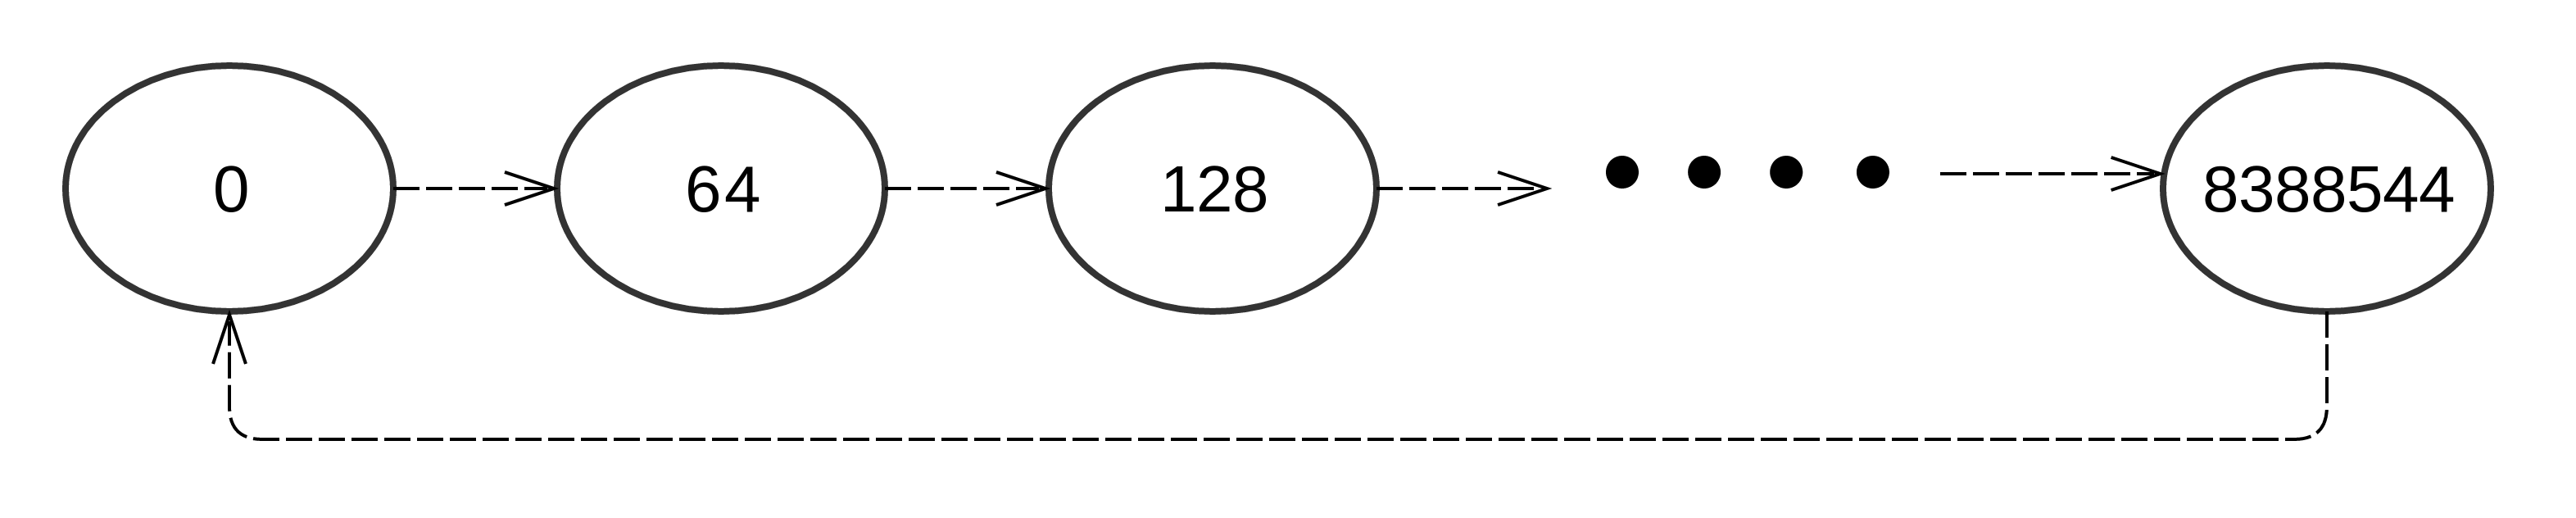
\includegraphics[width=\textwidth]{figures/circularlinkedlist.png}
\caption{Circular Linked List.}
\label{circularlinkedlist}
\end{figure}

The algorithm starts by accessing the buffer as a linked list, thus moving the contents of the buffer into the cache memory and bringing the cache into a known state. Then it measures the access time of a previously fixed variable, which now resides in RAM since the cache is filled with the buffer's contents. The script accesses the variable and measures the time it took to fetch it from RAM. Now the variable is located in the cache memory. The algorithm fetches the variable again and measures the time. The second access should be significantly faster since the variable was fetched from the cache memory.

The script collects multiple measurements by running the algorithm described above and depicted in Listing \ref{orenetal} multiple times. After obtaining the necessary data, the script plots the two sets of measurements as lines. I decided to collect measurements by running the algorithm 100 times. The resulted graph can be seen in Figure \ref{firefox39}.

The role of the website is to collect data by running the algorithm multiple times and plot the two sets. The success of the attack described by Oren et al. \cite{oren2015spy} is measured in how easily it is to distinguish between the two lines. If the graph shows two lines which do not intersect and there is a significant gap between them as in Figure \ref{firefox39} then an adversary could easily distinguish between a cache miss and a cache hit and the system is vulnerable to the cache attack \cite{oren2015spy}. On the other hand, if the graph looks more like Figure \ref{firefox45}, where plotting the time data does not give two non intersecting lines, then the machine is not affected by the aforementioned attack.

\begin{figure}[h]
\centering
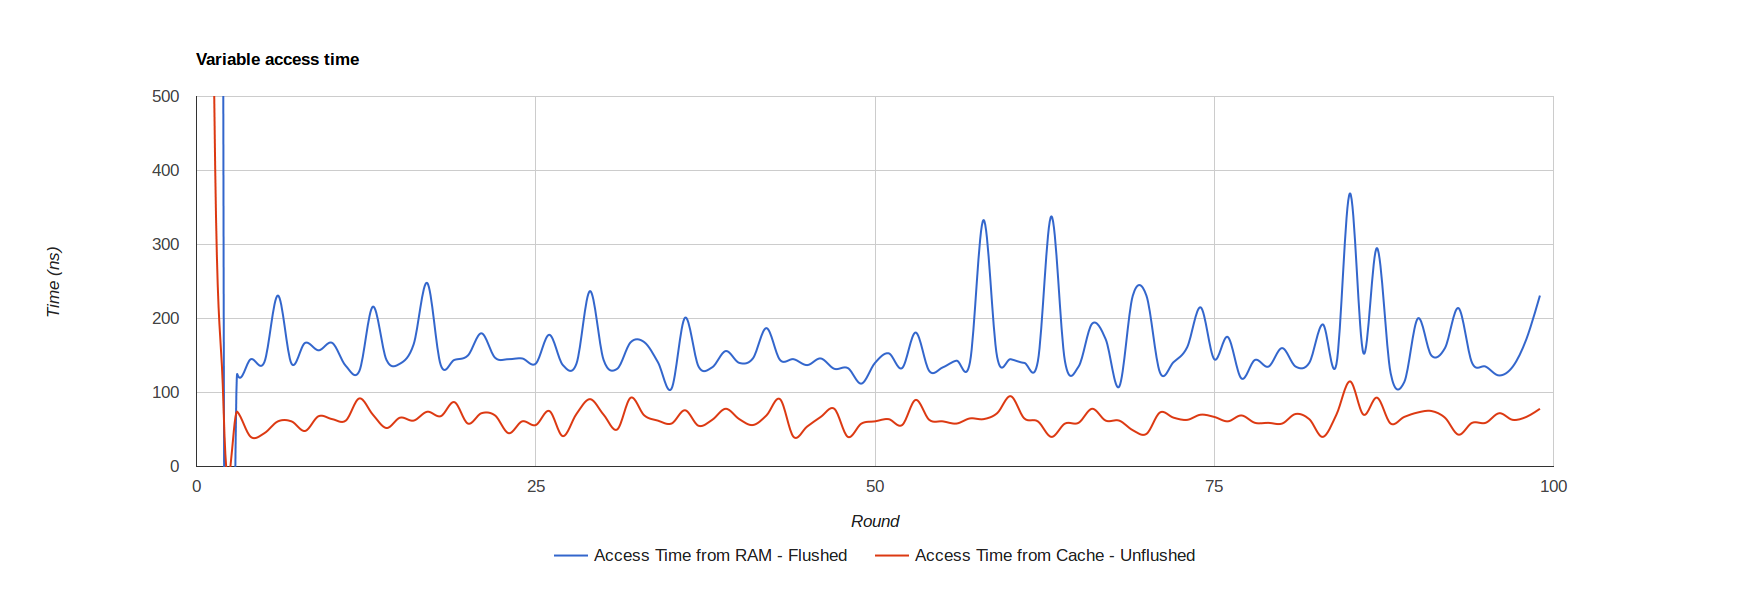
\includegraphics[width=\textwidth]{figures/firefox39.png}
\caption{Variable access times in Firefox 39.}
\label{firefox39}
\end{figure}

\begin{figure}[h]
\centering
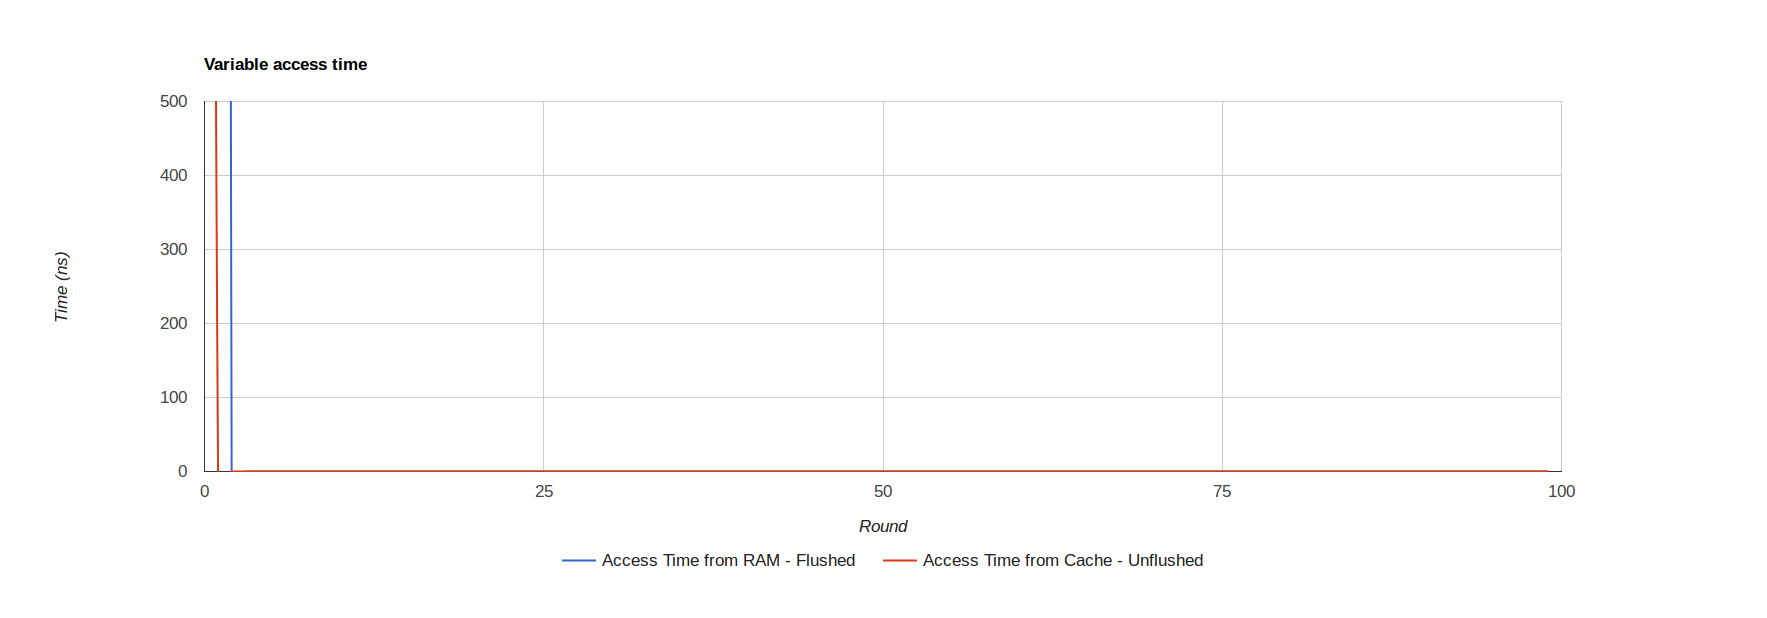
\includegraphics[width=\textwidth]{figures/firefox45.png}
\caption{Variable access times in Firefox 45.}
\label{firefox45}
\end{figure}

I discovered that the JavaScript High Resolution Time API has been updated in recent browsers and the measurements are not longer as precise as they used to be. The new version of the timing API provides time measurements accurate to a microsecond. If the difference between the time it takes to access a variable from the cache memory and from RAM is less than one microsecond (1000 nanoseconds), an adversary would not be unable to distinguish between the two values. In the attack presented by Oren et al. \cite{oren2015spy} the difference between the two values is on average under 100 nanoseconds, therefore browsers running the updated version of the API are no longer vulnerable to this attack. 

Figure \ref{firefox39} shows the two distributions, each represented as a line. As it can be seen, there is a clear difference in time between a variable accessed from RAM and one accessed from the cache memory. The timing data for Figure \ref{firefox39} was collected using Firefox 39. Figure \ref{firefox45} shows the same attack on the newest version of Firefox, Firefox 45, which contains the recent changes made to the JavaScript High Resolution Time API. The two distributions are indistinguishable, due to the loss in precision of the timing API, the two values are the same in most of the cases.

% rewrite nicer
%I have noticed that in the newest versions of Chrome and Firefox, the JavaScript High Resolution Time API provides time measurements accurate to 5 microseconds (5000 nanoseconds). Due to the small time difference between a cache hit and a cache miss (less than 100 nanoseconds) most of the time the two measurements map to the same value. Therefore the two lines overlap as it can be seen in Figure \ref{firefox45}.
 
%The change in the JavaScript timing API made the attack impossible in JavaScript as there are no known JavaScript APIs which provide the needed functionality. Also, browser vendors are aware of this attack and will not longer provide support for APIs which offer time measurements accurate to less than a microsecond. 
%
%Although the recent changes to the JavaScript High Resolution Time API makes the attack impossible in newer versions of the browser, there are still ways in which the attack can be implemented. Oren et al. decided to use JavaScript because it is the most popular client side language, therefore finding a vulnerability in JavaScript will affect a large number of user; however, there are other client side technologies which might still be affected by a similar attack. 

The attack was possible due to a feature of the JavaScript High Resolution Time API. Although, web applications do not require sub millisecond time measurements, the developers decided to include this feature in the API and browser vendors included the API in their products. Oren et al. were the first who thought about exploiting this feature and discovered that the an attacker could make use of the high precision time measurements provided by the API in order to obtain information about the state of the cache memory. They used this side channel information to compromise users' privacy by disclosing their browsing activity.
 
\section{JavaScript Timing Attacks}
\label{vanpe}
Van Goethem et al. \cite{van2015clock} present various methods for estimating the size of an external resource and claim that their techniques are faster and more accurate than previously used algorithms in similar timing attacks, such as the method presented by Bortz et al.\cite{bortz2007exposing}. In their paper, Van Goethem et al. \cite{van2015clock} propose the use of Video elements for loading an external resource as it provides more accurate time measurements than the Image method discovered by Bortz et al. \cite{bortz2007exposing}. Van Goethem et al. \cite{van2015clock}, also investigate how information leaked from newer technologies such as Application Cache and Service Workers can be used to track the users' browsing activity.

The attacks presented by Van Goethem et al. in \cite{van2015clock} are based on the assumption that an adversary can distinguish between files of different sizes only having access to the files' load times. I decided to test if several of the methods proposed in their paper are still possible and how accurately they can estimate the size of a cross-origin file. I built two web applications: one which compares the Video method proposed by Van Goethem et al. \cite{van2015clock} with the Image method presented by Bortz et al. \cite{bortz2007exposing} and tries to estimate the size of an external resource by loading it into a Video element, and a second application which estimates the size of a remote file using Service Workers.

The methods used by Van Goethem et al. \cite{van2015clock} to measure the loading time of a file from a cross-origin website require the files to be stored remotely. In order to test the attack, I set up a remote server, which contains randomly generated HTML files of different sizes ranging from 50kB to 1024kB. 

\subsection{Video vs. Image}
\label{vvsi}
Van Goethem et al. \cite{van2015clock} claim that loading a file into a Video element provides more accurate results than measuring the time by loading the file into an Image element. I built a web application which compares the two methods and also tries to estimate the size of an external resource using the Video algorithm proposed by Van Goethem et al. \cite{van2015clock}.

The web application can be split into two parts:
\begin{itemize}
\item A web page which lets users generate graphs in order to determine how easy it is to distinguish between files of different sizes by measuring the load time using either the Video or the Image methods which can be seen in Figure \ref{fig:videointerface}.
\item And a second web page which tries to estimate the size of a given file by using the Video method proposed by Van Goethem et al. in \cite{van2015clock}. The web page can be seen in Figure \ref{fig:videoguess}.
\end{itemize}

The two web pages communicate with a background script which provides the time measuring methods and generates all the data needed for plotting the graph. The script is written entirely in JavaScript. The front-end was built using AngularJS\cite{angularjs} , whose two way data binding simplifies the process of sending data between the background script and the front end parts of the application.

\subsubsection{Back-end}

The back-end script contains various functions for measuring the time of loading an external resource into an Image element or a Video element. The algorithm for measuring the loading time of an external resource as a video is presented in Listing \ref{vanvideo}. The JavaScript code for measuring the time it take to load a file as an Image is presented in Listing \ref{vanimage}.

The Image method was first proposed by Bortz et al. in \cite{bortz2007exposing}, where it was used to estimate the size of a cross-origin resource. The value returned by this method measures the total time it takes to download the external resource, which is highly dependent on the network conditions. 

The function from Listing \ref{vanimage} starts by creating a new Image object, which will hold the contents of the file whose size we are trying to guess. Before setting the value of the \texttt{src} attribute, the \texttt{error} event needs to be registered on the Image object. The \texttt{error} event fires when the browser is unable to display the resource as an image, which usually happens as soon as the file has finished downloading. 

\begin{lstlisting}[caption={Measuring the load time of an external resource as an Image},label={vanimage}]
function measureTimeImage(url) {
    return new Promise(function(resolve, reject) {
        var img = new Image();
        img.onerror = function() {
            var end = window.performance.now();
            var time = end-start;
            resolve(time);
        }
        var start = window.performance.now();
        img.src = url;
    });
};
\end{lstlisting}

The JavaScript High Resolution Time API described in Section \ref{javascript}, which provides time measurements accurate to one microsecond, is used to measure the loading time. The original algorithm, proposed by Bortz et el \cite{bortz2007exposing}, was using the \texttt{Date.now()} \cite{datenow} method to measure the time, which returns the number of milliseconds elapsed since 1 January 1970 00:00:00 UTC. The JavaScript High Resolution Time API measures the time elapsed since the page has started loading. This method of estimating time, provides better measurements, which are relative to the page and are not influenced by changes in the system's time. The API contains a single method, \texttt{performance.now()}, which returns the number of microseconds elapsed since the pages has started loading.

To measure the time it takes to load the resource, we call the \texttt{performance.now()} method in order to receive the time elapsed since the application started loading and store the value in a variable, \texttt{start}. Then we set the value of the \texttt{src} attribute to link which points to the file we are trying to estimate the size of. The browser will start downloading the resource and once it received all the data will try to display it. In case the resource is not a valid image file, the \texttt{error} event will fire. We know that the \texttt{error} event is only triggered once the file has finished downloading so we measure the time again by calling the \texttt{performance.now()} method, and store the value in \texttt{end}. The time difference between the two variables, \texttt{end} and \texttt{start}, represents the total load time of the file. The function ends by returning the time measurement.

The function, which measures the load time of a file as an image, returns a promise, which will be resolved to the time measurement value. A JavaScript promise represents an action which has not completed yet, but is expected to in the future. Promises are used to make sure that the current file has completely finished downloading before any other operation is started. 

Promises are needed as the script might reach the end before the browser has finished downloading the external resource. When the \texttt{measureTimeImage()} method is called, JavaScript will not wait for a value to be returned from the \texttt{error} event ,but will move on and set the expected value to \texttt{undefined}. When multiple measurements are being collected, we need a way to make sure that the previous time measurement has been recorded before calling the function again.  
Initially, I was calling the \texttt{measureTimeImage()} method from inside the \texttt{error} event, similar to a recursive call; however, using JavaScript Promises makes the code neater and easier to read.

Measuring the time it takes to load a file as an Image is dependent on the network conditions and is heavily influenced by loss of packets and server load. Van Goethem et al. \cite{van2015clock} propose replacing the Image element with a recently introduced HTML element, the Video element. They claim that this method provides more accurate results since the time measurement is independent of the network conditions. The function used for measuring the time it takes to load a cross-origin file into a video element is presented in Listing \ref{vanvideo}.

Similarly to the Image object, the Video object has an \texttt{error} event associated, which fires when the browser learns that the file to be displayed is not a valid video file. The video element has some additional events, which can be monitored, such as \texttt{progress} and \texttt{suspend}. The \texttt{progress} event is being triggered periodically while the file is being downloaded. Once the file has finished downloading, the \texttt{suspend} event will fire. 

The \texttt{error} event associated with the Video element has a slightly different behaviour than the one from the Image element. Additionally, it is known to act differently between browser versions. In Chrome, the \texttt{error} event will fire once the browser has finished parsing the contents of the file and it realizes the resource is not a valid video file. Therefore, the time between the \texttt{suspend} event and the \texttt{error} event is dependent on the size of the file. Firefox, however, does not wait until it has finished parsing the contents of the file and will trigger the \texttt{error} event as soon as the resource has finished downloading, if the file is not valid. Despite the video method only working in Chrome, it is still worth mentioning since, according to \cite{statcounter}, over half of the world's desktop and tablet users use Chrome.

\begin{lstlisting}[caption={Measuring the load time of an external resource as a Video},label={vanvideo}]
function measureTimeVideo(url) {
	return new Promise(function(resolve, reject) {
		var video = document.createElement('video');
        // The error is triggered when the file has finished parsing.
		video.onerror = function() {
			timeError = window.performance.now();
			var time = timeError - timeSuspend;
			resolve(time);
		};
		// Start timing once the resource is loaded and parsing begins.
		video.onsuspend = function() {
			timeSuspend = window.performance.now();
		};
		var timeSuspend, timeError;
		video.src = url;
	});
};
\end{lstlisting}

The function described in Listing \ref{vanvideo} returns a promise which resolves to the time measurement once the browser has finished parsing the resource. The function starts  by creating a new Video object which will contain the contents of the cross-origin resource. Again, the events we are monitoring need to be registered before we set the value of the \texttt{src} attribute. Compared to the Image object, where only one event was being watched, for the Video object we are going to use two events, \texttt{error} and \texttt{suspend}.

After the needed events are registered on the Video object, the function declares a couple of variables, \texttt{timeSuspend} and \texttt{timeError}, which will be used to store the time when the downloading process has started and when it ended. Then, it sets the value of the \texttt{src} attribute to the url where the external resource resides. Once the \texttt{src} attribute is set the browser starts downloading the cross-origin resource and triggers the \texttt{progress} event. The \texttt{progress} event does not need to be watched since it does not provide any information which can help estimate the size of the external resource. 

The \texttt{suspend} event will fire once the browser has finished downloading the file. This event is being triggered after the file has finished downloading, but before the browser has started the parsing process. In Listing \ref{vanvideo}, when the \texttt{suspend} event fires, the \texttt{performance.now()} method is called in order to obtain the current time stamp and the values is stored in \texttt{timeSuspend}. Then the browser starts the parsing process, which depending on the browser version can be interrupted by the \texttt{error} event as soon as the browser starts parsing in Firefox, or when the browser has finished parsing the contents of the file in Chrome. 

I used Chrome as the default browser for testing the attacks described by Van Goethem et al. \cite{van2015clock} so I am going to focus on the behaviour of the \texttt{error} event in this browser. Once the browser has finished parsing the recently downloaded file it tries to display it. The \texttt{error} event will fire if the resource is not a valid video file. When the event fires, a call will be made to the \texttt{performance.now()} method in order to obtain the time since the page has started loading. Again, we store the time measurement in a variable, \texttt{timeError}.

The difference between the two variables, \texttt{timeError} and \texttt{timeSuspend}, represents the time it took the browser to parse the contents of the file, which is dependent on the size of the file. Once the \texttt{error} event fires, the function computes the time value and resolves the promise.

As it can be seen from the description of the two functions presented in Listing \ref{vanimage} and Listing \ref{vanvideo}, there is a significant difference in the way they measure the load time of the file. The Image method measures how long it takes to download the resource, which can be influenced by network conditions, while the Video method measures how long it takes the browser to parse the contents of the resource. Due to varying network conditions in the case of the Image method and noise produced by other processes running on the same system in the Video method case, multiple time measurements need to be collected in order to accurately estimate the size of the file. 

The first method I implemented for collecting multiple time measurements for the same file was simply to call one of the functions in Listing \ref{vanimage} or Listing \ref{vanvideo} multiple times. If data from multiple files was needed, we call the previous method for each given file. Web servers might block a website if they receive too many requests. Web browsers can stop the script if they notice that the same request is being sent multiple times. Therefore, the previously described method of collecting multiple measurements does not always work. 

Additionally, web browsers might cache the response if the same resource is being requested numerous times, which can affect the Image method as it measures the download time. If the resource is cached, the Image method would measure the time it takes to read the response from the browser's cache memory. Although the time it takes to read a file from the browser's cache is dependent on the size of the file, there is no way to tell if the resource is served from the browser's cache or over the network. Thus, when requesting the file multiple times we can end up with some of the values representing retrieval from cache and the rest of the values representing download time. The video method is not affected by caching. Moreover, the total runtime of the attack using the video method will improve since most of the time is wasted on re-downloading the cross-origin files. 

The second method alternates the requests such that no consecutive request have the same data, therefore the browser is less likely to cache the resources and the remote server should not be able to detect the attack. The method can be used when multiple time measurements are needed from at least two different files. This method collects one time measurement for each given file, then shuffles the files and repeats the process until enough data has been gathered. 

Apart from providing methods for collecting data, the back-end script also deals with creating the graphs. The application uses the Google Charts API to draw the graphs. An example of a graph can be seen in Figure \ref{fig:videointerface}.


\subsubsection{Graph}

\begin{figure}[h]
\centering
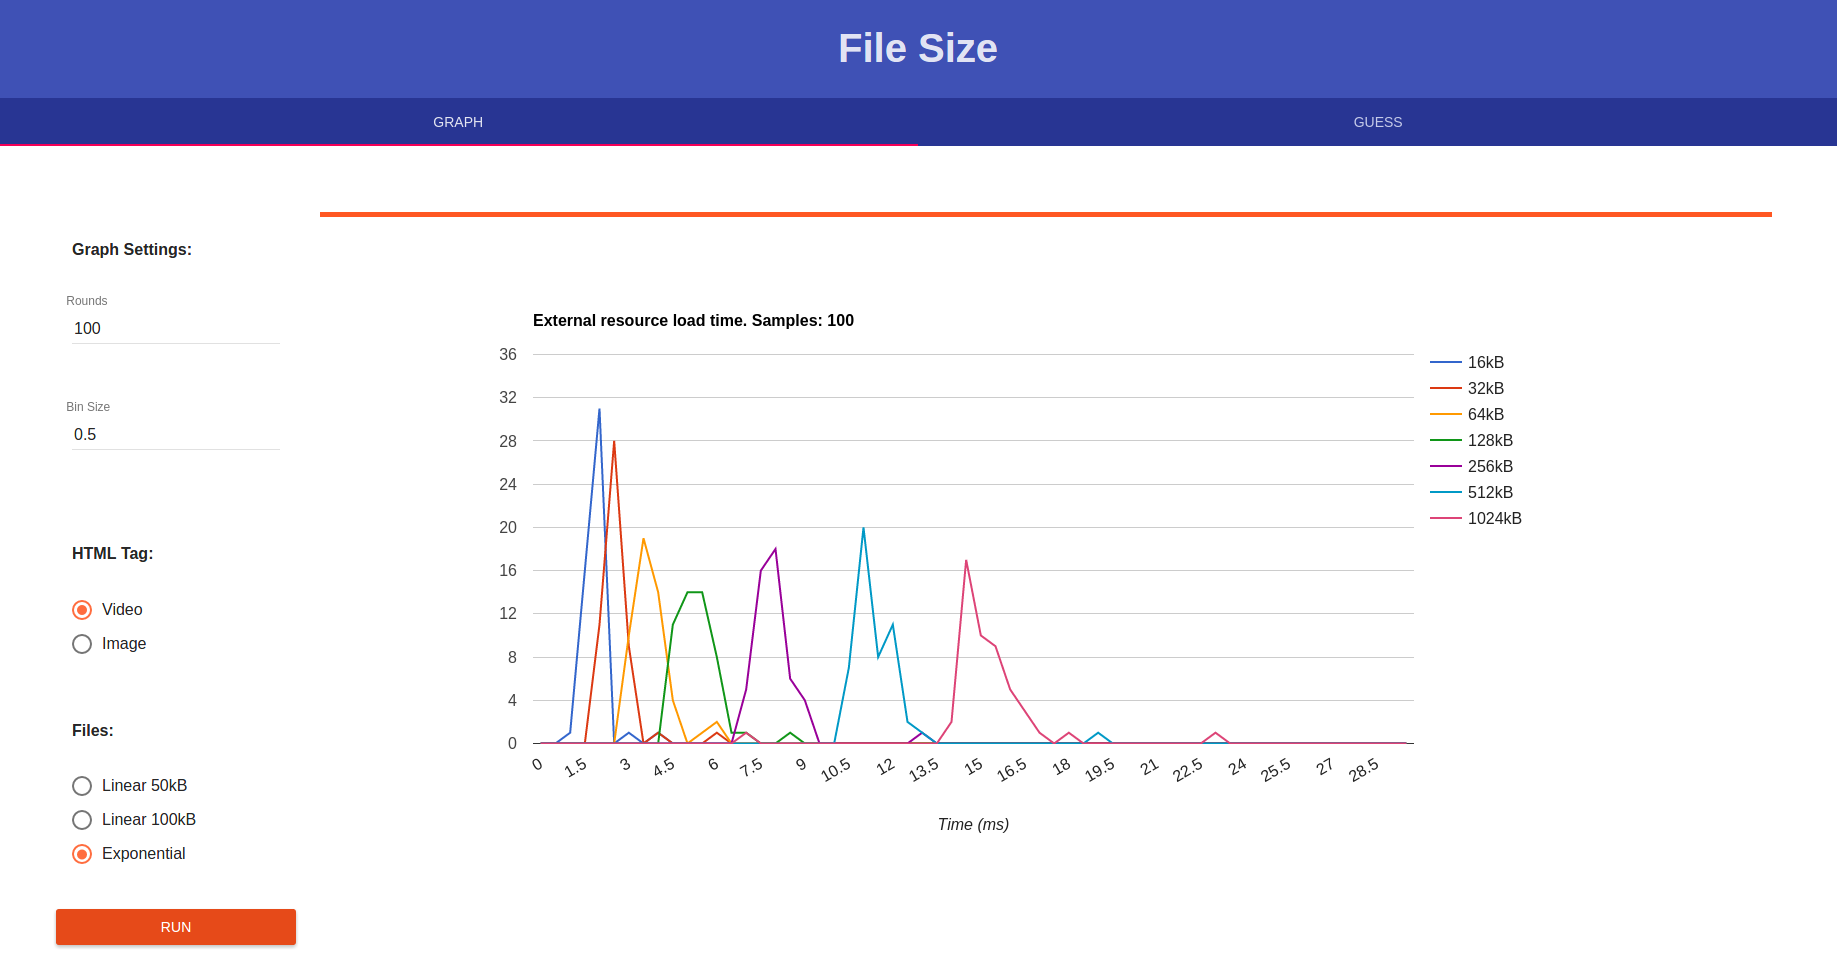
\includegraphics[width=\textwidth]{figures/interface.png}
\caption{Web application interface for creating graphs.}
\label{fig:videointerface}
\end{figure}

The Graph generating part provides a user friendly interface as it can be seen in Figure \ref{fig:videointerface}. On the left side there is a dashboard which lets the user customize the graph. They can choose from three different data sets:
\begin{itemize}
\item The first group contains 10 files with sizes ranging from 100kB to 1000kB, in 100kB increments.
\item The second group contains 10 files with sizes ranging from 50kB to 500kB, in 50kB increments.
\item The third group contains 7 files with sizes: 16kB, 32kB, 64kB, 128kB, 256kB, 512kB and 1024kB.
\end{itemize}

The application provides two method for measuring the load time the files: video described in Listing \ref{vanvideo}, and audio described in Listing \ref{vanimage}. Users can also change the number of measurements to be recorder for each file, by default the application gathers 50 time measurements for each of the files in the data set. There is also an option for selecting the bin size for the plot.

\begin{lstlisting}[caption={JavaScript implementation of the Fisher-Yates algorithm},label={fisheryates}]
function shuffle(array) {
	for(var counter=array.length-1; counter > 0; counter--) {
		var index = Math.floor(Math.random() * counter);
		var temp = array[counter];
		array[counter] = array[index];
		array[index] = temp;
	}
	return array;
};
\end{lstlisting}

After setting all the parameters, a user has to click the \texttt{RUN} button in order to generate the graph shown on the right side in Figure \ref{fig:videointerface}. The button calls a JavaScript function, which collects all the user provided information such as what data set to use, how many measurements to collect, what method to use for measuring the loading time and the bin size. The function constructs an object with all the needed information and sends it to the function responsible for collecting the time measurements.

The function receives a list of files for which it has to collect multiple time measurement using the shuffling technique described in the previous section. The function shuffles the files, measures the time it takes to load each of the files one and repeats the process until enough data has been collected. The list of files is shuffled using the Fisher-Yates algorithm \cite{fisher1949statistical} defined in Listing \ref{fisheryates}. After all the necessary data has been collected, the script calls the graph drawing function. The set of measurements for each file is presented as a histogram.  

\subsubsection{Guess}

The second part of the web application estimates the size of a given file. The user provides the URL to a cross-origin resource, such as a Facebook profile page or a random HTML file and the application uses the Video method presented in Listing \ref{vanvideo} to guess the size of the file.

\begin{figure}[h]
\centering
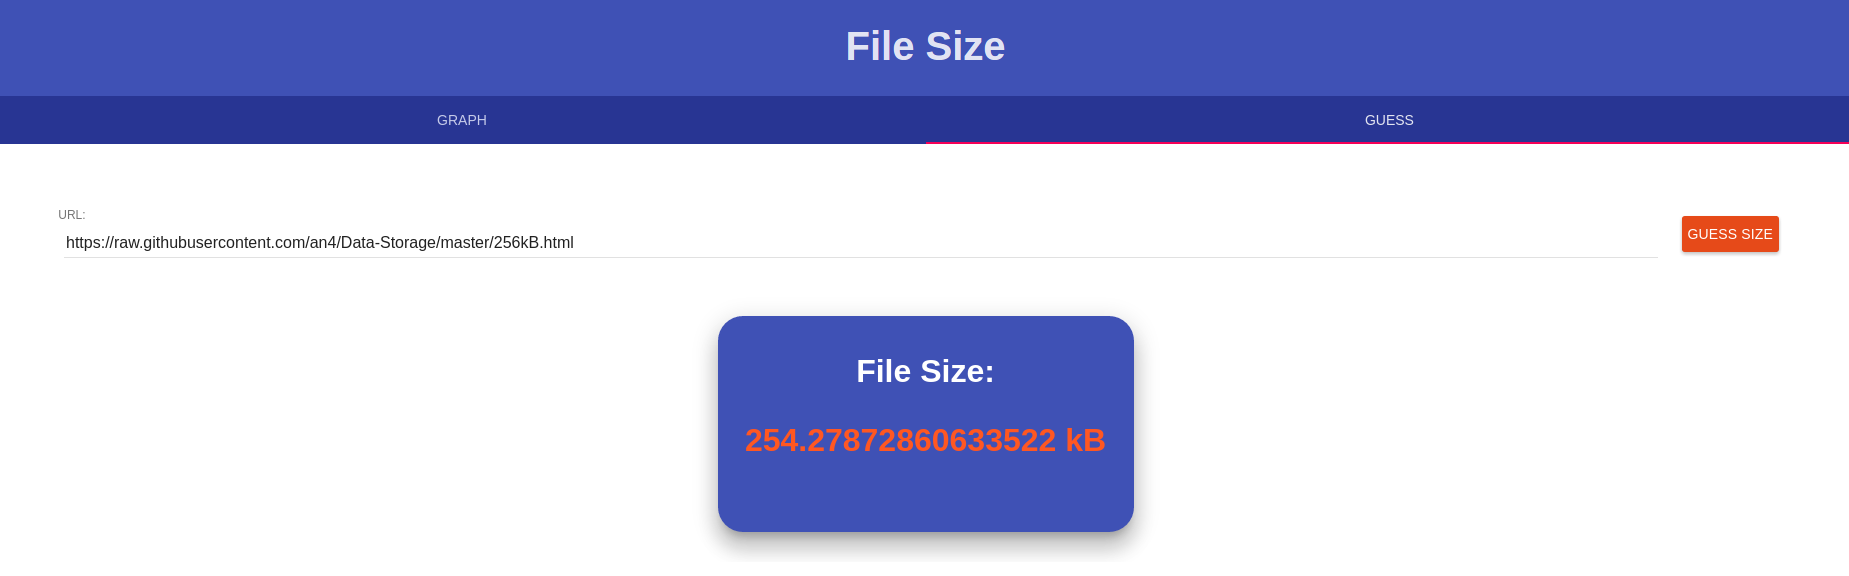
\includegraphics[width=\textwidth]{figures/guess.png}
\caption{Web application interface for estimating size of file.}
\label{fig:videoguess}
\end{figure}

In order to estimate the size of a file, a user has to type the URL pointing to the file's location in the input box and click the \texttt{GUESS SIZE} button. Once the button is clicked a function on the back end side will fetch the URL and start the guessing process.

The function collects multiple measurements by calling the function presented in Listing \ref{vanvideo} multiple times. The time measurements can be influenced by noise produced by the victim's system, we select the minimum value since it is the least likely to have been influenced by noise. 

\begin{lstlisting}[caption={JavaScript code for estimating the size of a cross-origin file.},label={filesizevideo}]
function guessSize(unknownFileLoadTime, load100, load200) {
	var size = 0;
	if(unknownFileLoadTime > load100) {
		unknownFileLoadTime -= load100;
		size += 100;
		size = size + 100 * (uunknownFileLoadTime/(load200-load100));
	}
	return size;
};
\end{lstlisting}

Another problem we face when trying to determine the size of a file from a cross-origin website is that there is no way to determine what system the victim is using, they can browse the website from a mobile device or a laptop. The time measurement obtained by running the \texttt{measureTimeVideo()} method is influenced by the system the website is being accessed from. In order to determine the victim's system speed we are going to measure the load time of two files of known sizes (100kB and 200kB). The files reside on the remote server we set up earlier in order to compare the two measurement methods. We collect multiple time measurements for the two files and choose the minimum values, as they are less influenced by noise.

Subtracting the time it takes to parse the 100kB file  from the time it takes to parse the 200kB , gives us the time it takes to parse a chuck of 100kB of a file. I decided to use the difference between the two measurements to obtain the time it takes to parse 100kB, rather than use the time it takes to parse the 100kB file, since the parsing process spends some time opening the file. We use the following algorithm presented in Listing \ref{filesizevideo} to determine the size of the file.

The function receives the time it takes to parse the unknown file, the times it takes to parse the 100kB and 200kB files. The function is only able to guess the size of files whose actual size is greater than 100kB; however, the parameter's of the function can easily be changed such that it supports files of different sizes. If the time it takes to load the unknown file is less than the time it takes to parse the 100kB file, we return zero. Otherwise we calculate the size of the file as it can be seen in Listing \ref{filesizevideo} and return the resulted value. The result is going to be displayed on the web page in the box located at the bottom of Figure \ref{fig:videoguess}.

\subsection{Application Cache}

The Video method proposed by Van Goethem et al. \cite{van2015clock} re-downloads the file before every measurement. This increases the overall run-time of the attack since it requires the collection of numerous time measurements for each file. In their paper, they propose the use of Application Cache. AppCache allows resources to be stored locally and be served from local storage when they are requested. 

The files to be cached need to be specified in a manifest file and included in the header of the main HTML file. The first time the web application is opened, the browser will download the resources and store them in the browser's cache for an unlimited time. Van Goethem et al. \cite{van2015clock} observed an overall speed up of the attack when using the AppCache mechanism to store the files locally and then fetch them from local storage before each measurement.

\subsection{Service Worker}
\label{webSW}

Measuring the load time of an external resource when loading it as a Video only works in Chrome. Van Goethem et al. \cite{van2015clock} also used Service Workers in order to determine the size of a cross-origin file. Service Workers are event driven Web Worker which are able to overwrite default network behaviour. They are supported in all mainstream browsers (Chrome, Firefox, Safari). I build another web application, which estimates the size of a given file using Service Workers. The web site can be seen in Figure \ref{fig:swguess}.

A Service Worker is a background script, which runs independent of the main web application. Service Workers do not have access to the main application and cannot manipulate the DOM; however, they can communicate with the main application through messages. The website consists of two scripts: a main script which deals with gathering the information from the user and displaying the results, and a Service Worker which monitors network requests and estimates the size of the hidden data.

\begin{figure}[h]
\centering
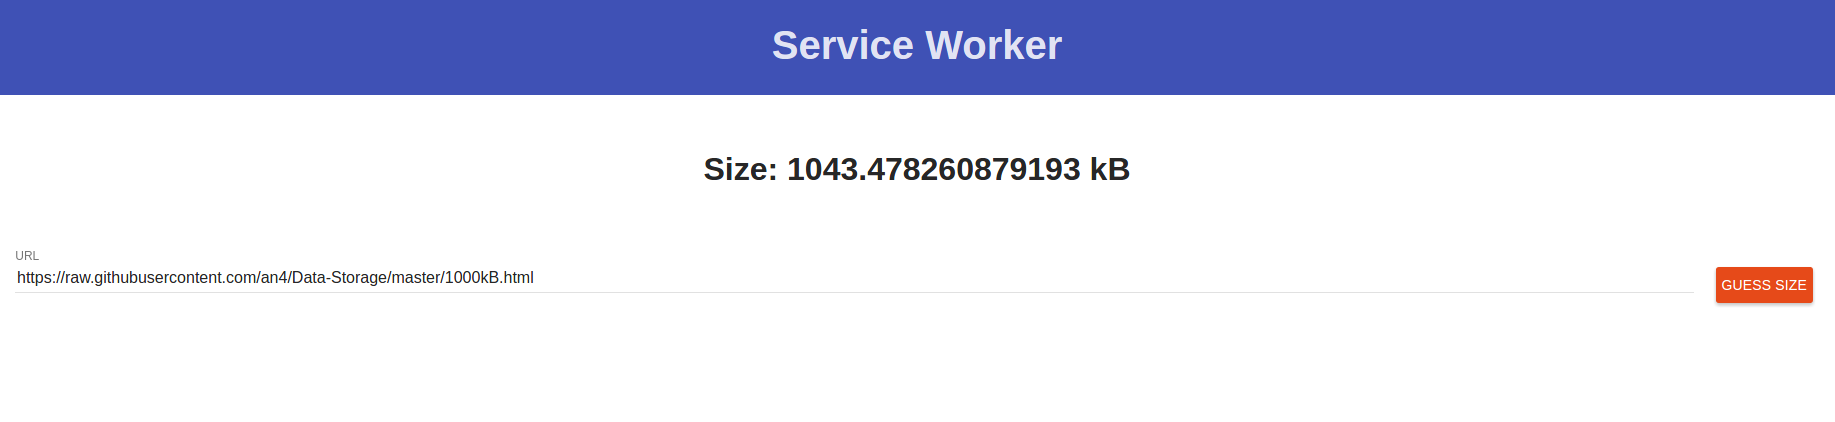
\includegraphics[width=\textwidth]{figures/sw_size.png}
\caption{Web application interface for estimating size of file using Service Workers.}
\label{fig:swguess}
\end{figure}

The main script is responsible for monitoring the user interaction with the application front-end shown in Figure \ref{fig:swguess}. The user can type a URL in the input field and click the \texttt{GUESS SIZE} button, which will call a function the \texttt{guessSize()} method from the main script. The \texttt{guessSize()} method, shown in Listing \ref{SWimg}, takes the input from the user and tries to load it into an Image object. Once the \texttt{src} attribute on the Image object is set, the browser will send a request to download the external resource. Since the Service Worker is already registered and monitors all network requests made by the page, the request made from \texttt{guessSize()} will be detected by the Service Worker script.

% where are SW used, introduce Cache Api, cant see the hidden request but we can measure the time it takes to write to cache, again dependent on the system rather than the network

\begin{lstlisting}[caption={Loading file as an Image},label={SWimg}]
$scope.guessSize = function() {
	var img = new Image();
	img.src = $scope.sw.url;
};
\end{lstlisting}

The Service Worker script will catch the fetch request and start the process of estimating the file size. Although, Service Workers are generally used to provide an offline version of web applications, they do not automatically store every request the detect in order to serve it from local memory later. Service Workers use the Cache API \cite{cacheAPI} to store all the resources they might need when there is no network connection.

\begin{lstlisting}[caption={JavaScript code for measuring the time it takes to write to cache.},label={putdelete}]
function putDelete(url, response, cache) {
    return new Promise(function(resolve, reject) {
        var end;
        var start = performance.now();
        cache.put(url, response.clone()).then(function() {
            end = performance.now();
            var time = end-start;
            cache.delete(url).then(function(res) {
                resolve(time);
            });
        });
    });
};
\end{lstlisting}

In their paper Van Goethem et al. \cite{van2015clock} use the time it takes to write the response to the cache memory as a side channel in order to estimate the size of the hidden data. The Cache API stores (key, value) pairs, where the key is the URL provided by the user, and the value is the response object returned by the Fetch API. The JavaScript function for measuring the time it takes to add the response to cache is presented in Listing \ref{putdelete}. 

The \texttt{putDelete()} method add a key, value pair to cache, measures the time it takes to store the data into the cache object and then removes it from cache. The function uses the JavaScript High Resolution Time API presented in Section \ref{javascript} to measure the time it takes to store the response into the cache object. The Cache API provides methods for adding an object to cache, \texttt{put}, and removing an element from the cache, \texttt{delete}. Both these methods return a promise, which can either be resolved when the operations is successful or rejected an error occurs during the add or remove operations.  

The script collects numerous measurements by calling the \texttt{putDelete()} function multiple times and chooses the smallest time value as it is least likely to have been altered by noise. The script is unable to determine the victim's system so we need to compare the time it takes to store the unknown file against files with known size. The application measures the time of storing two files: one of 100kB and one of 200kB, and uses the obtained values to determine the size of the hidden data. The function for determining the cross-origin resource's size can be seen in Listing \ref{SWsize}. The two variables, \texttt{time100} and \texttt{time200}, represent the time it takes to store the 100kB and 200kB files, and \texttt{time} is the time returned after calling the \texttt{putDelete()} method on the unknown file. Once it has calculated the size of the hidden file, the Service Worker sends the result to the main script in order to be displayed as it can be seen in Figure \ref{fig:swguess}.

\begin{lstlisting}[caption={JavaScript code for estimating the size of a file.},label={SWsize}]
var size = 0;
if(time > time100) {
    time -= time100;
    size += 100;
    var timeStep = time200 - time100;
    var x = time/timeStep;
    size = size + 100 * x;
}
\end{lstlisting}

\subsection{Critical Evaluation}

\subsubsection{Video vs. Image}

The first application I built in order to test the attacks discovered by Van Goethem et al. \cite{van2015clock} compares the efficiency of two methods for estimating the size of a file from a cross-origin website. The first method was proposed by Bortz et al. \cite{bortz2007exposing} and measures the time it takes to load an external resource as an Image object, which represents the total download time of the file. The second method was discovered by Van Goethem et al. \cite{van2015clock} and uses the time it takes to load a file from a cross-origin website into a \texttt{video} element to estimate the size of the hidden data. The method used by Van Goethem et al. \cite{van2015clock} measures the time it takes the browser to parse the file, which is dependent on the system on which the website is running rather than network conditions, like in the case of the method proposed by Bortz et al. \cite{bortz2007exposing}. Van Goethem et al. \cite{van2015clock} claim that their method provides more accurate timing measurement. I am going to test this claim by comparing the results obtained by the two methods on different data sets.

The efficiency of the two methods is measures in how easily it is to distinguish between files of different sizes. If plotting the data, results in a graph where the distributions of the time measurements for each file do not overlap, then an attacker could easily distinguish between files of different sizes and they will be able to obtain private information about the user. On the other hand, if when plotting the data, the distributions overlap, an attacker would be unable to accurately determine the size of a given file.

I created three different data sets in order to test the two methods:
\begin{itemize}
\item Data Set 1: contains 10 files with sizes ranging from 50kB to 500kB, in 50kB increments.
\item Data Set 2: contains 10 files with sizes ranging from 100kB to 1000kB, in 100kB increments.
\item Data Set 3: contains 7 files with sizes: 16kB, 32kB, 64kB, 128kB, 256kB, 512kB, 1024kB.
\end{itemize}

I used the web application described in Section \ref{vvsi} to generate six graphs, which are going to help compare the efficiency of the two methods. Figure \ref{fig:l50V} and Figure \ref{fig:l50I} were obtained by timing the load time of the files from the first data set. The first graph is using the Image method proposed by Bortz et al. \cite{bortz2007exposing}, while the second image, Figure \ref{fig:l50V} uses the Video methods discovered by Van Goethem et al. \cite{van2015clock}.

As it can be seen from the two figures, Figure \ref{fig:l50V} and Figure \ref{fig:l50I}, the video methods performs better as the time measurements of the different files are easily distinguishable. In Figure \ref{fig:l50I} the data contains values which are very close, making it almost impossible to distinguish between files of different sizes. The Video method performs slightly better, especially for the four smallest files (50kB, 100kB, 150kB and 200kB); however, as the size of the files gets bigger is becoming very hard to distinguish between them.

\begin{figure}[h]
\centering
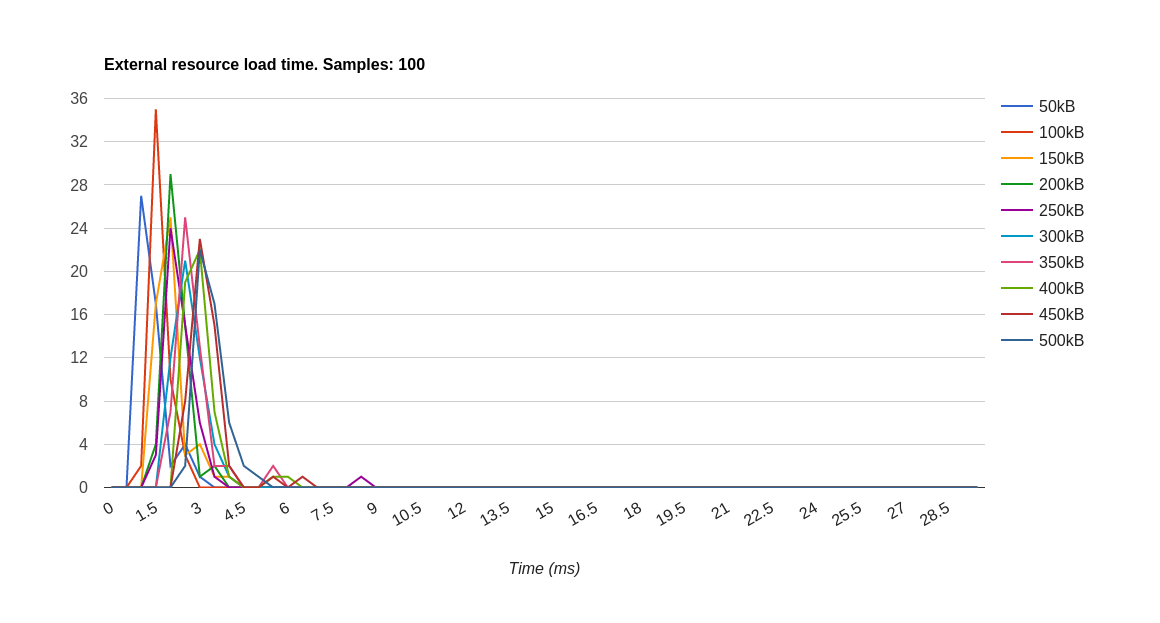
\includegraphics[width=\textwidth, height=7cm]{figures/i100L50H.png}
\caption{Data Set 1 - Image}
\label{fig:l50V}
\end{figure}

\begin{figure}[h]
\centering
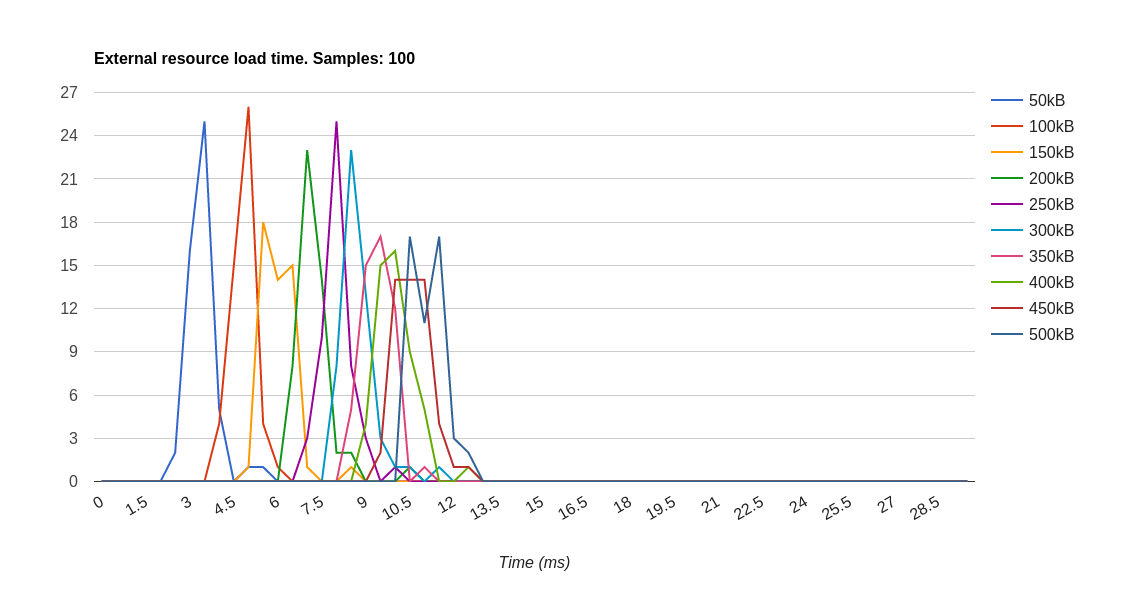
\includegraphics[width=\textwidth, height=7cm]{figures/v100L50H.png}
\caption{Data Set 1 - Video}
\label{fig:l50I}
\end{figure}

I decided to run the same experiment on a different data set, with files ranging from 100kB to 1000kB, in 100kB increments. The results of the experiment can be seen in Figure \ref{fig:l100V} for the Video method, and in Figure \ref{fig:l100I} for the Image method. As expected, the Video method provided slightly better results; however, it is still hard to distinguish between files of larger size. This is due to the fact that the absolute difference between two consecutive files remains constant, 100kB, as the file sizes increase, while the difference between them compared to the actual file size decreases. For example, it is easier to distinguish between two files, one of 100kB and one of 200kb, since the second one is double the size of the first one. Whereas, when the sizes of the files are 900kB and 1000kB, the size of the second file is only 11\% bigger than the size of the first file.

The image method performed better on the second data set, where the difference between the two consecutive files is 100kB, compared to the first data set. This behaviour was expected since the download times is dependent on the size of the file.

\begin{figure}[h]
\centering
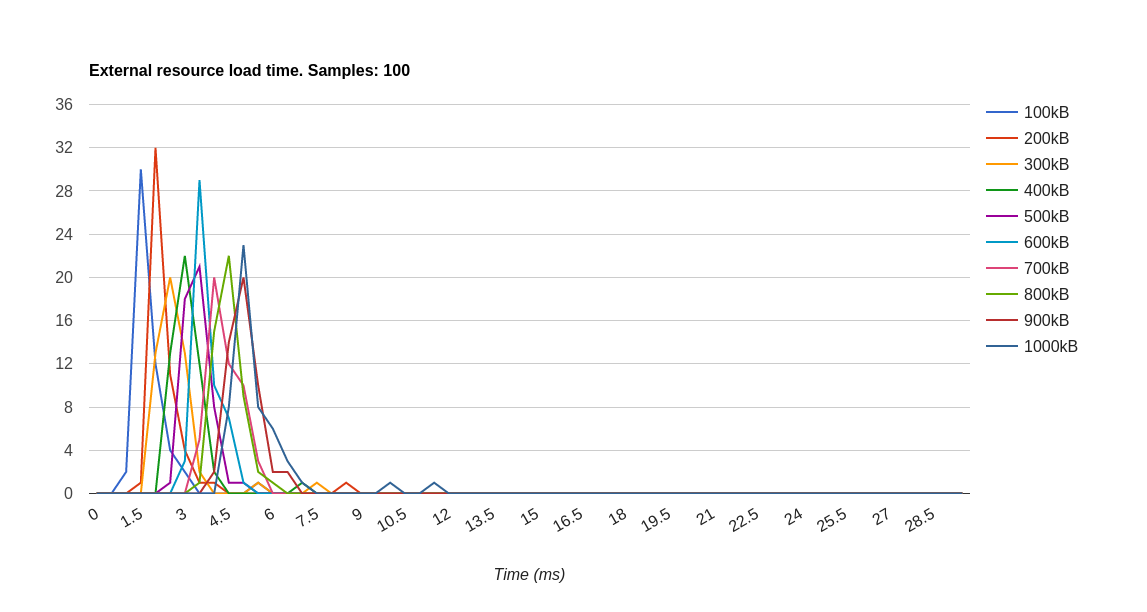
\includegraphics[width=\textwidth, height=7cm]{figures/i100L100.png}
\caption{Data Set 2 - Image}
\label{fig:l100V}
\end{figure}

\begin{figure}[h]
\centering
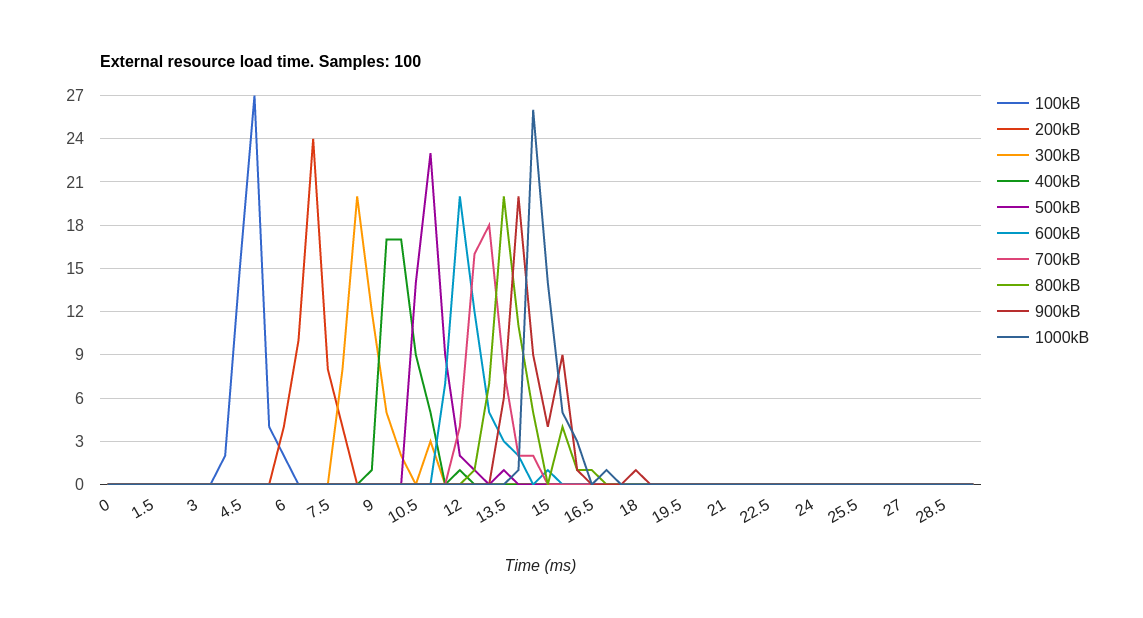
\includegraphics[width=\textwidth, height=7cm]{figures/v100L100.png}
\caption{Data Set 2 - Video}
\label{fig:l100I}
\end{figure}

The last data set I tested the two methods on contains file whose sizes increase logarithmically, the difference between two consecutive files does not remain constant as the file size increases. The difference between the files in this data set, should fix the problem we had earlier where as the file sizes increase it is very hard to distinguish between files of different sizes. 

The results of running the experiment on the third data set are shown in Figure \ref{fig:eV} for the video method and in Figure \ref{fig:eI} for the image method. As expected, when plotting the data obtained from loading the files as videos, there is a clear difference between all the files in the data set and and adversary could easily distinguish between them. 

As before, the Image method produced inconclusive results. It is impossible to distinguish between the smaller files. Surprisingly, the difference between the two larger files, 512kB and 1024kB, is quite obvious. Therefore an attacker would be able to differentiate between files of different sizes using the image method, as long as the difference in size between the two files is at least 500kB.

\begin{figure}[h]
\centering
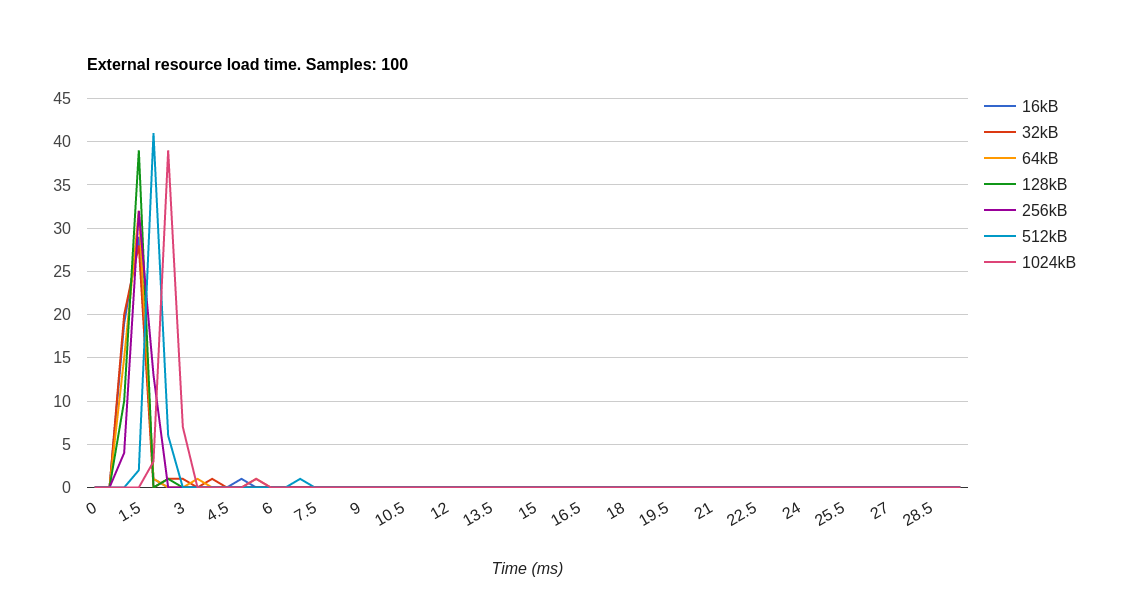
\includegraphics[width=\textwidth, height=7cm]{figures/i100E.png}
\caption{Data Set 3 - Image}
\label{fig:eV}
\end{figure}

\begin{figure}[h]
\centering
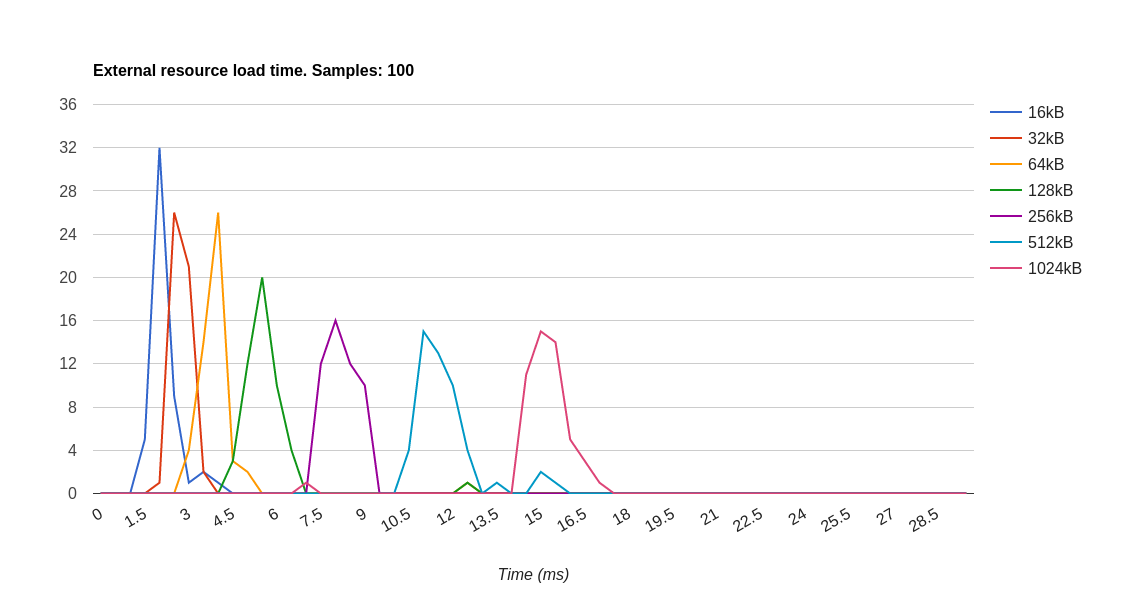
\includegraphics[width=\textwidth, height=7cm]{figures/v100E.png}
\caption{Data Set 3 - Video}
\label{fig:eI}
\end{figure}

From the six resulted graphs after running the experiment three times it is obvious that the video method provides better results than the image method and it can be used by an attacker to distinguish between files of different sizes. It is easy to distinguish between two files as long as their size of the bigger file is at least 25\% greater than the size of the smaller file, in the case of the video method. 

From the graphs it can be seen that the image method is generally faster than the video method; however, this is due to running the experiments on a fairly stable network with fast internet access. It is expected that the average user will have a less stable and slower connection which will produce different graphs for the image method. The distribution for each file will have a larger standard deviation and the means will shift to the right as the speed of the connection decreases. Even if the network conditions change it is very unlikely that an attacker would be able to distinguish between files of similar sizes using the image method.

After using the graph side of the application to compare the video method with the image method on different data sets, I decided to test how accurately the guess part of the web application estimates the size of a file. 

I chose four files of different sizes and run the guess function five times for each file. The results obtained from running the experiment are presented in Table \ref{tab:guessVideo}. For the table it can be seen that the function for estimating a file size implemented using the video method does not work for larger files. 

\begin{table}[t]
\centering
\begin{tabular}{|c|c|c|c|c|c|}
\hline
\textbf{File Size} & \textbf{Guess 1} & \textbf{Guess 2} & \textbf{Guess 3} & \textbf{Guess 4} & \textbf{Guess 5} \\
\hline
$200$ kB & $198$ kB & $200$ kB & $201$ kB & $196$ kB & $202$ kB \\
\hline
$400$ kB & $360$ kB & $378$ kB & $377$ kB & $382$ kB & $379$ kB \\
\hline
$600$ kB & $470$ kB & $480$ kB & $450$ kB & $461$ kB & $470$ kB \\
\hline
$800$ kB & $541$ kB & $520$ kB & $634$ kB & $545$ kB & $587$ kB \\
\hline
\end{tabular}
\caption{Estimation the size of a file using the video method}
\label{tab:guessVideo}
\end{table}

\subsubsection{Application Cache}
Although, using AppCache improves the speed of the attack and increases the chances of success if the attacker has a short time frame to gather all the needed information, the Application Cache framework is no longer supported by mainstream browsers. AppCache has numerous disadvantages which determined developers to start using a similar technology, Service Workers.

\subsubsection{Service Worker}

I decided to test the performance of the website described in Section \ref{webSW} by estimating the size of ten files of different sizes ranging from 100kB to 1000kB. The results of the experiment can be seen in Table \ref{tab:guessSW}. There were five measurements collected for each file. As it can be seen from the table, the size of the files estimated by the web application is very close to the actual size of the files.

\begin{table}[h]
\centering
\begin{tabular}{|c|c|c|c|c|c|}
\hline
\textbf{File Size} & \textbf{Guess 1} & \textbf{Guess 2} & \textbf{Guess 3} & \textbf{Guess 4} & \textbf{Guess 5} \\
\hline
$100$ kB & $100$ kB & $126$ kB & $141$ kB & $100$ kB & $125$ kB \\
\hline
$200$ kB & $165$ kB & $199$ kB & $173$ kB & $207$ kB & $195$ kB \\
\hline
$300$ kB & $258$ kB & $307$ kB & $275$ kB & $246$ kB & $362$ kB \\
\hline
$400$ kB & $541$ kB & $520$ kB & $634$ kB & $545$ kB & $587$ kB \\
\hline
$500$ kB & $558$ kB & $521$ kB & $454$ kB & $488$ kB & $459$ kB \\
\hline
$600$ kB & $705$ kB & $567$ kB & $533$ kB & $654$ kB & $603$ kB \\
\hline
$700$ kB & $646$ kB & $776$ kB & $721$ kB & $731$ kB & $696$ kB \\
\hline
$800$ kB & $700$ kB & $912$ kB & $795$ kB & $844$ kB & $724$ kB \\
\hline
$900$ kB & $750$ kB & $860$ kB & $821$ kB & $998$ kB & $1009$ kB \\
\hline
$1000$ kB & $855$ kB & $1105$ kB & $1067$ kB & $971$ kB & $1114$ kB \\
\hline
\end{tabular}
\caption{Estimation the size of a file using Service Workers}
\label{tab:guessSW}
\end{table}

% -----------------------------------------------------------------------------

\chapter{Conclusion}
\label{chap:conclusion}

The aim of this dissertation is to review some of the most important side-channel attacks, which affect browser software, discovered over the past twenty years. Throughout the course of this dissertation I present some of the attacks, test if they can still be performed today or how efficient the given countermeasures are in preventing the attacks. Additionally, I analyse the performance of two recent side-channel attacks, one using the browser's cache memory to disclose a user's browsing activity, the other one using timing information in order to estimate the size of hidden data.

Browser use a wide range of technologies in order to display richer, more interactive and responsive web applications. These technologies leak side channel information which can be used to disclose private data about users. Felten et al. \cite{felten2000timing} showed that it is possible to determine what resources are in a user's cache. Jia et al.\cite{jia2015know} use a similar technique to derive a user's location. More recently, Bortz et al.\cite{bortz2007exposing} proved that they can estimate the size of a hidden file by simply checking how long it takes to download the resource. The browser's cache memory is not the only source of leakage, Clover\cite{cssvisited} demonstrated that he can determine what pages a user has visited by requesting the computed style.

Van Goethem et al. \cite{van2015clock} extend the work of Bortz et al. \cite{bortz2007exposing} and present four new techniques for estimating the size of a cross-origin resource: loading the data into a \texttt{<video>} element, loading the data into a \texttt{<script>} element, using Service Workers to measure the time it takes to write the data to local storage and measuring the time it takes to load the file from cache after being stored locally using Application Cache. Van Goethem et al. \cite{van2015clock} claim that their methods are more efficient than the measuring technique discovered by Bortz et al. \cite{bortz2007exposing}. 

I investigated their claims and discovered that the methods proposed by Van Goethem et al.\cite{van2015clock} perform better and are generally faster, since they require less measurements, than previously used time measuring techniques, such as the one proposed by Bortz et al.\cite{bortz2007exposing}. Since the release of their paper, browsers have started removing support for Application Cache, due to its limited functionality, therefore the attack they present using AppCache is no longer possible. Out of the four measurement techniques presented in Van Goethem et al.'s \cite{van2015clock} paper, the only one which still affects all the mainstream browsers is the measurement technique which uses Service Workers. 

% Oren part
Oren et al.\cite{oren2015spy} propose e browser cache timing attack which analyses the state of the browser's cache memory in order to disclose a user's browsing activity. Their attack uses the PRIME+PROBE algorithm, which was first used to recover the secret parameters in AES\cite{pub2001197}, in to determine the state of the victim's cache memory. Compared to other cache timing attacks, Oren et al.'s \cite{oren2015spy} attack tracks the user's behaviour rather than the disclosure of private data. The attack is written in JavaScript and runs entirely in the browser. The choice of programming language for implementing the attack, allowed the researchers to target a wider range of people since the requirement for running the attack are limited. 

The attack proposed by Oren et al.\cite{oren2015spy} is possible due to a faulty implementation of the JavaScript High Resolution Time API\cite{jshighresolutiontimeapi}. The JavaScript High Resolution Time API is a fairly recent feature of JavaScript which provides sub millisecond time measurements. The motivation behind the API is to allow developers to better analyse the performance of their applications, which was not possible using previous time measuring methods like \texttt{Date.now()}\cite{datenow}. Oren et al.\cite{oren2015spy} discovered that the measurements provided by the API are precise enough to distinguish a cache miss from a cache hit which led to the previously mentioned attack which discloses a user's browsing activity.

Oren et al.'s \cite{oren2015spy} is based on the assumption that an attacker can distinguish between a cache hit and a cache miss with high probability, which is possible due to the existence of the JavaScrip High Resolution Time API. The API has been recently updated such that it provides measurements up to a microsecond, which is no longer enough to distinguish between a cache hit and a cache miss. Although, the attack is no longer possible in recent version of the mainstream browser due to the change in the timing API, there might be other APIs available which provide time measurements accurate to a nanosecond.

To conclude, browser attacks are an important category of side-channel attacks which pose an imminent threat to the privacy of online users. Side-channel information obtained through running browser attacks can be used to disclose private information about the user, such as their location, browsing history and in some cases their current browsing activity.






















%One of the oldest side-channel attacks, targeting browser software, was discovered by Felten and Schneider \cite{felten2000timing} in 2000. Their attack, uses timing information on order to determine if a resource resides in the victim's browser cache. This information enabled them to determine what web pages the user has visited, therefore revealing a user's browsing history. Although, there have been various countermeasures proposed, the attack is still possible. Researchers believe that the best defence against the attack is the use of the same-origin policy on the browser's cache memory; however, browser vendors are against implementing this feature since it might slow down the browser software. 
%
%Another attack which discloses the user's browsing history was discovered by Clover \cite{cssvisited} around the same time. This attack uses the fact that the majority of browsers change the style of a visited link such that users can keep track of what websites they visited. Clover discovered that an attacker can request the computed style of the page using JavaScript. This technique has been used for over a decade by high profile websites in order to obtain the users' browsing history. The attack was fixed by changing the implementation of the JavaScript function which returns the web page's computed style. 
%
%Jia et al. \cite{jia2015know} showed that it is possible to determine a user's country, city and even neighbourhood by simply checking the state of their browser's cache memory. Their paper uses the technique presented by Felten and Schneider \cite{felten2000timing} together with the fact that some websites offer location specific web pages in order to improve the user's experience. There are no known countermeasures against this type of attack. Jia et al. suggest that websites should only offer geo-specific services if they have the user's explicit permission.
%
%Targeting static HTML pages is not the only way to obtain private information about a user. Bortz et al. \cite{bortz2007exposing} were the first to show that it is possible to estimate the amount of data a user has access to. They introduced two new categories of browser attacks: \textit{direct timing} attacks and \textit{cross-site timing} attacks. In direct timing attacks, the attacker has direct access to the website and uses the web server's response time in order to disclose private information about the website. The second category, cross-site timing attacks, the attacker tries to gain access to the victim's view of another website. Bortz et al. \cite{bortz2007exposing} present a new method for estimating the size of a cross-origin file; however, their technique is dependent on the network speed and stability. The researchers discovered that by loading a file as an image it is possible to measure the total download time, which is dependent on the size of the file. Therefore, they were able to estimate the size of hidden data by simply measuring how long it takes to load an external resource into an \texttt{<img>} element.
%
%Van Goethem et al. \cite{van2015clock} extend the work of Bortz et al. \cite{bortz2007exposing} and present four new techniques for estimating the size of a cross-origin resource: loading the data into a \texttt{<video>} element, loading the data into a \texttt{<script>} element, using Service Workers to measure the time it takes to write the data to local storage and measuring the time it takes to load the file from cache after being stored locally using Application Cache. 
%
%Van Goethem et al. \cite{van2015clock} claim that their methods are more efficient than the measuring technique discovered by Bortz et al. \cite{bortz2007exposing}. In Section \ref{vanpe} I analyse the efficiency of the four methods and compare the video method to the image method presented in \cite{bortz2007exposing}.
%
%I tested the two methods, video and image, on three different data sets, and in all three of the cases the video method proposed by Van Goethem et al. \cite{van2015clock} performed better. Therefore, the claim made by Van Goethem et al. \cite{van2015clock} is true. The video method measures the time it takes the browser to parse the file, whereas the image method measures the download time of the resource, which is influenced by the network connection. I discovered that the attack which estimates the size of an external resource by loading it into a \texttt{<video>} element only works in Chrome.
%
%The second measurement method proposed by Van Goethem et al. \cite{van2015clock} was the use of Application Cache. AppCache described in Section \ref{applicationcachetb}, allows the developer to cache some of the resources in order to be served later from local storage. The researches use the AppCache together with the video method in order to speed up the overall runtime of the attack by avoiding re-downloading the resource before every measurement and loading it from local storage instead. Apart, from reducing the overall runtime of the attack the use of Application Cache provides no additional benefit. Additionally, the mainstream browsers starting removing support for AppCache, as there are better technologies available, such as Service Workers, which offer similar functionality.
%
%Another measurement technique used by Van Goethem et al. \cite{van2015clock} to determine the size of a cross-origin resource is measuring the time it takes to write a file to local storage using Service Workers and the Cache API. Out of all the methods in their paper \cite{van2015clock} this one provides the best results when estimating the size of an external resource. Additionally, is the only one who is supported by all mainstream browsers, therefore an attack using Service Workers will affect more users.
%
%The last measurement method presented in the paper uses measures the time it takes to load the resource as a script. Although Van Goethem et al. \cite{van2015clock} claim that this technique has been around for a long time I have been unable to recreate their attack using the \texttt{<script>} element. It seems that the browser checks if the file is valid before it starts the download process, therefore the timing information does not disclose anything about the file's size.





%%%%%%%%%%%%%%%%%%%%%%%%%%%%%%%%%%%%%%%%%%%%%%%%%%%%%%%%%%%%%%%%%%%%%%%%%%%%%%%%%%%%%%%%
%%%%%%%%%%%%%%%%%%%%%%%%%%%%%%%%%%%%%% The End %%%%%%%%%%%%%%%%%%%%%%%%%%%%%%%%%%%%%%%%%
%%%%%%%%%%%%%%%%%%%%%%%%%%%%%%%%%%%%%%%%%%%%%%%%%%%%%%%%%%%%%%%%%%%%%%%%%%%%%%%%%%%%%%%%

%============================================================================================
% Back Matter

\cleardoublepage
\pagestyle{marked}

\bibliographystyle{ieeetr}
\bibliography{main.bib}

\end{document}
